\documentclass[a4paper,openright,12pt]{book}

\usepackage[spanish]{babel}
\usepackage[utf8]{inputenc}
\usepackage{enumerate}
\usepackage{url}
\usepackage{graphicx}
\graphicspath{ {./img/} }
\usepackage{wrapfig}
\usepackage{a4wide}
\usepackage{html}
\usepackage{hthtml}
\usepackage{listings}
\usepackage{multirow}
\usepackage{lscape}

\usepackage[font={footnotesize,it}]{caption}
\usepackage[normalsize]{subfigure}
\usepackage{color}
\usepackage[usenames,dvipsnames,svgnames,table]{xcolor}
\usepackage{amsmath}

\pretolerance=10000
%Para que no corte las palabras al final de la linea.

\DeclareGraphicsExtensions{.png,.jpg,.pdf,.eps}
\usepackage{geometry}
\geometry{a4paper, left=2.6cm, right=2.2cm, top=3.0cm, bottom=3.0cm}

\linespread{1.3}

\setlength{\parskip}{1ex plus 0.5ex minus 0.2ex}

%listings style
\definecolor{mygreen}{rgb}{0,0.6,0}
\definecolor{mygray}{rgb}{0.5,0.5,0.5}
\definecolor{mymauve}{rgb}{0.58,0,0.82}
\definecolor{lightgray}{rgb}{.9,.9,.9}
\definecolor{darkgray}{rgb}{.4,.4,.4}
\definecolor{purple}{rgb}{0.65, 0.12, 0.82}

\lstset{
	language=xml,
	tabsize=3,
	label=code:sample,
	frame=shadowbox,
	rulesepcolor=\color{gray},
	xleftmargin=20pt,
	framexleftmargin=15pt,
	keywordstyle=\color{blue}\bf,
	commentstyle=\color{OliveGreen},
	stringstyle=\color{red},
	numbers=left,
	numberstyle=\tiny,
	numbersep=5pt,
	breaklines=true,
	showstringspaces=false,
	basicstyle=\footnotesize,
	emph={model, name, static, link, pose, collision, geometry, mesh, scale, uri, visual},emphstyle={\color{magenta}}
}

\begin{document}
	
	
	
	
	
	
% Para que salga la bibliografia en el indice
\let\OLDthebibliography=\thebibliography
\def\thebibliography#1{\OLDthebibliography{#1}%
	\addcontentsline{toc}{chapter}{\bibname}}

\tableofcontents
\listoffigures
	
	
\chapter{Introducción}
\label{ch:Introduccion}
\pagenumbering{arabic} 

En este proyecto se construirá material docente para la enseñanza de robótica utilizando diversas tecnologías. Para saber cual es el marco de desarrollo y dónde se engloban los conceptos utilizados vamos a introducir algunos términos que servirán como contexto y que permitirán entender mejor de dónde surge la necesidad de estos escenarios y la utilidad de los mismos.

\section{Robótica}
\label{sec:intr_robotica}

Según la Wikipedia\cite{wikipedia}, \textit{La robótica es la rama de la ingeniería mecatrónica, de la ingeniería eléctrica, de la ingeniería electrónica, de la ingeniería mecánica, de la ingeniería biomédica y de las ciencias de la computación que se ocupa del diseño, construcción, operación, disposición estructural, manufactura y aplicación de los robots.}

Otra definición menos técnica podría ser: La robótica es una ciencia o rama de la tecnología, que estudia el diseño y construcción de máquinas capaces de desempeñar tareas realizadas por el ser humano o que requieren del uso de inteligencia. Por tanto, estamos ante una ciencia que se encarga de diseñar máquinas que sean capaces de reemplazar al ser humano en algunas acciones. Es una disciplina con sus propios problemas, sus fundamentos y sus leyes, y podemos observar dos vertientes de la misma, la teórica y la práctica. En la parte teórica podemos agrupar todas las aportaciones de la informática, la inteligencia artificial y la automatización. En cuanto a la parte práctica observamos aportaciones relativas tanto a la construcción del robot como a la de su gestión, siendo por tanto destacadas las aportaciones de la mecánica, electrónica, programación, etc. Esto hace de la robótica una ciencia con un marcado carácter interdisciplinario.

\subsection{Historia de la robótica}
\label{subsec:intr_historiarobotica}

La historia de la robótica ha estado unida a la construcción de “artefactos”, que trataban de materializar el deseo humano de crear seres semejantes a nosotros que nos descargasen del trabajo. Desde los primeros pasos de la civilización el ser humano ha desarrollado ingenios tanto para facilitar sus labores como para imitar a la naturaleza, fascinando a sus congéneres. De los antiguos egipcios se conservan descripciones de más de 100 máquinas y autómatas, (incluyendo un artefacto con fuego, un órgano de viento, una máquina operada mediante una moneda, una máquina de vapor) en la obra \textit{Pneumática y Autómata} de Herón de Alejandría. Los griegos nos dejaron creaciones como un pájaro de madera, a vapor, que fue capaz de volar, y genios como Leonardo da Vinci el diseño de un \textit{Caballero mecánico}. 

En el año 1921 un escritor checo, Karel Capek, publica su obra \textit{“Los Robots Universales de Rossum”}, en la que aparece por primera vez la palabra “robot“ derivada de la palabra checa robota, que significa servidumbre o trabajo forzado. Unos años más tarde, en 1942, la revista americana \textit{Astounding Science Fiction} pública "Círculo Vicioso" (Runaround en inglés), una historia de ciencia ficción escrita por Isaac Asimov donde aparecen por primera vez las Tres leyes de la robótica. Estas leyes establecen lo siguiente:
\begin{quote}
\begin{enumerate}[1.ª]
	\item Un robot no hará daño a un ser humano o, por inacción, permitir que un ser humano sufra daño.
	\item Un robot debe hacer o realizar las órdenes dadas por los seres humanos, excepto si estas órdenes entrasen en conflicto con la 1ª Ley.
	\item Un robot debe proteger su propia existencia en la medida en que esta protección no entre en conflicto con la 1ª o la 2ª Ley.
\end{enumerate}
\end{quote}

Pese a que son fruto de una obra de ciencia ficción, estas leyes han dado la vuelta al mundo y multitud de científicos e investigadores las toman como ciertas, siendo un concepto que aún hoy tiene sentido para los futuros desarrollos en torno a sistemas autónomos. La autonomía de las máquinas debería acompañarse de medidas de seguridad que evitaran el daño a las personas. Esto es un precepto que las tres leyes de la robótica de Asimov contienen. De hecho, la idea del escritor era proteger al ser humano, que los robots, por muy avanzados que estuvieran, no pudieran volverse contra las personas. En el caso de un coche autónomo, si este conduce sin pasajeros dentro y va a chocar contra otro donde viajan varias personas, ¿debe el primer vehículo echarse a un lado aunque esté circulando correctamente y vaya a sufrir más daños si lo hace? La primera ley de Asimov diría que sí. En cuanto a la segunda ley, actualmente no se concibe el desarrollo de ningún sistema autónomo sin mecanismos que permitan a las personas manejarlos manualmente, y se considera que aún no existe un sistema tan fiable y preciso como para darle mayor autoridad que al ser humano que lo controla. En el año 1982 Isaac Asimov publicó \textit{El robot completo} (The Complete Robot en inglés), una colección de cuentos de ciencia ficción escritos entre 1940 y 1976. En esta colección vuelve a explicar las tres leyes de la robótica con más ahínco y complejidad moral. Incluso llega a plantear la muerte de un ser humano por la mano de un robot con las tres leyes programadas, por lo que decide incluir una cuarta ley "La ley 0 (cero)": \textit{Un robot no hará daño a la Humanidad o, por inacción, permitir que la Humanidad sufra daño}.

\begin{wrapfigure}{l}{0.3\textwidth}
	\centering
	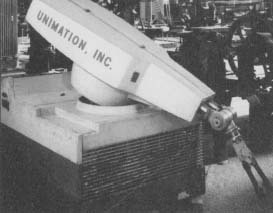
\includegraphics[width=0.2\textwidth]{unimation.jpg}
	\caption{Robot de Unimation usado por Ford en 1961.} \label{fig:unimation}
\end{wrapfigure}
En la década de 1950 se comienzan a desarrollar los primeros robots comerciales. En 1956 se comercializa el primer robot de la compañía Unimation, fundada por George Devol y Joseph Engelberger. En 1961 se instala en una fábrica de la Ford Motors Company uno de estos robots (\textit{Figura \ref{fig:unimation}}), cuya función era la de levantar y apilar grandes piezas de metal caliente. En 1971 el “Standford Arm“, un pequeño brazo robótico de accionamiento eléctrico, se desarrolló en la Standford University. En 1973 la empresa Kuka\footnote{\url{https://www.kuka.com/}} desarrolla el primer robot industrial con seis ejes electromecánicos, el Famulus. 

Pero la robótica no se basa sólo en las máquinas que revolucionaron los procesos industriales, el concepto de robótica incluye y cada vez se orienta más hacia los sistemas móviles autónomos, que son aquellos capaces de desenvolverse por sí mismos en entornos desconocidos sin necesidad de supervisión. Con esta idea en mente, en los setenta, la NASA inicio un programa de cooperación con el Jet Propulsión Laboratory para desarrollar plataformas capaces de explorar terrenos hostiles. El primer fruto de esta alianza sería el Mars-Rover, que estaba equipado con un brazo mecánico tipo Standford, un dispositivo telemétrico láser, cámaras estéreo y sensores de proximidad. Sin embargo, fue la Unión Soviética en 1971 la primera en lograr aterrizar un robot en la superficie de marte con éxito, el Mars 3, aunque la comunicación se perdió minutos después. No fue hasta 1976 que la NASA hizo llegar al primer robot estadounidense a Marte, el Viking I. En la Figura \ref{fig:vikingmars} podemos observar tanto el Mars-Rover como el Viking.

\begin{figure}[t]
	\centering
	\subfigure[Mars 3]{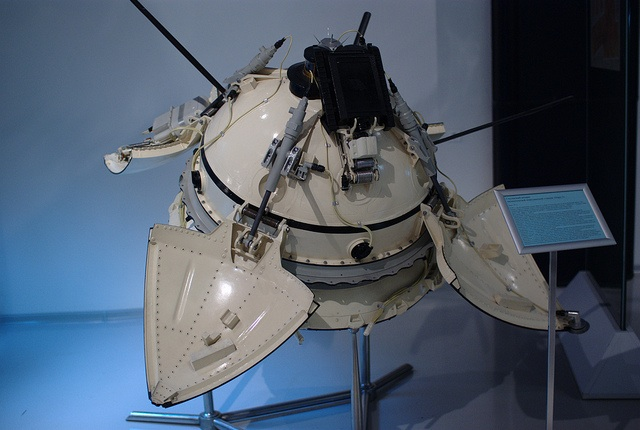
\includegraphics[width=0.4\textwidth]{mars3.jpg}}\hspace{0.05\textwidth}
	\subfigure[Viking I]{\includegraphics[width=0.4\textwidth]{viking1.jpg}}
	\caption[Los primeros robots espaciales, el Mars 3 y el Viking I]{Imágenes de los primeros robots espaciales: una copia del Mars 3 (a) expuesto en el Museo Memorial de la Cosmonáutica en Moscú, y en Dr. Carl Sagan posando junto a un modelo del Viking I (b) en el Valle de la Muerte, California} \label{fig:vikingmars}
\end{figure}

Desde entonces la robótica ha experimentado en multitud de aplicaciones y formatos con modelos sumamente ambiciosos, como es el caso del IT, diseñado para expresar emociones, el COG, también conocido como el robot de cuatro sentidos, el famoso Sojourner o el Lunar Rover, vehículos con control remoto, y otros mucho mas específicos como el Cypher, un helicóptero robot de uso militar, el guardia de trafico japonés Anzen Taro o los robots mascotas de Sony. En el campo de los robots antropomorfos (androides) se debe mencionar el P3 de Honda que mide 1.60m, pesa 130 Kg y es capaz de subir y bajar escaleras, abrir puertas, pulsar interruptores y empujar vehículos, así como el robot ASIMO de la misma compañía, capaz de desplazarse de forma bípeda e interactuar con las personas.

En general la historia de la robótica la podemos clasificar en cinco generaciones (división hecha por Michael Cancel, director del Centro de Aplicaciones Robóticas de Science Application Inc. en 1984): 
\begin{enumerate}[1.ª Generación]
	\item[1.ª Generación] Robots manipuladores. Son sistemas mecánicos multifuncionales con un sencillo sistema de control, bien manual, de secuencia fija o de secuencia variable.
	\item[2.ª Generación] Robots de aprendizaje. Repiten una secuencia de movimientos que ha sido ejecutada previamente por un operador humano. El modo de hacerlo es a través de un dispositivo mecánico. El operador realiza los movimientos requeridos mientras el robot le sigue y los memoriza.
	\item[3.ª Generación] Robots con control sensorizado. El controlador es una computadora que ejecuta las órdenes de un programa y las envía al manipulador para que realice los movimientos necesarios.
	\item[4.ª Generación] Robots inteligentes. Son similares a los anteriores, pero además poseen sensores que envían información a la computadora de control sobre el estado del proceso. Esto permite una toma inteligente de decisiones y el control del proceso en tiempo real.
\end{enumerate}

Las dos primeras, ya fueron alcanzadas en los ochenta. La tercera generación, que incluye visión artificial, ha avanzado mucho en los ochenta y noventa. La cuarta contempla movilidad avanzada en exteriores e interiores. Y podríamos hablar incluso de una quinta, en la cual entrarían los más modernos sistemas de aprendizaje autónomo y la inteligencia artificial.

El campo de la robótica está en constante expansión, y su popularidad aumenta rápidamente. Ya no solo vemos grandes avances en los robots industriales, como en cadenas de producción, envasado de alimentos o gestión de almacenes, sino que los robots domésticos están cobrando cada vez más importancia. El éxito de los robots aspiradora como Roomba de iRobot\footnote{\url{http://www.irobot.es/}}, la incorporación de aparcamiento automático en coches de todas las gamas o incluso asistentes de conducción autónoma como el autopiloto de Tesla\footnote{\url{https://www.tesla.com/es_ES/}} o prototipos de Google o Apple, los diversos modelos de robots desactivadores de explosivos de los cuerpos de seguridad del mundo, el sistema quirúrgico Da Vinci que permite incluso operar siendo teleoperado desde otro país, los grupos de robots coordinados usados en construcción o misiones de búsqueda y rescate, termostatos inteligentes como el Nest\footnote{\url{https://nest.com/thermostat/meet-nest-thermostat/}} de Google, o la inmensa variedad de drones del mercado ponen de manifiesto que ésta es una tendencia en auge a nivel global.

\begin{figure}[h]
	\centering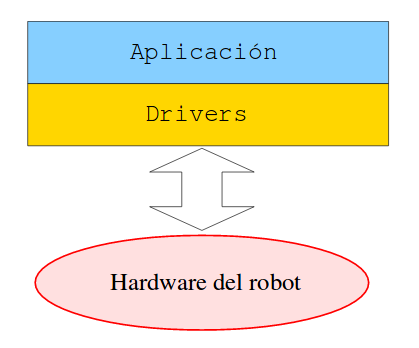
\includegraphics[width=0.5\textwidth]{esquemarobot.png}
	\caption{Esquema básico del funcionamiento de un robot.}
	\label{fig:esquemarobot}
\end{figure}

Viendo el esquema común a cualquier robot (\textit{Figura \ref{fig:esquemarobot}}), uno de los factores que permiten diseñar, construir y comercializar los robots asegurando una inteligencia y robustez ante situaciones reales es la programación que hay detrás de estos, su software. Usualmente este software tiene varias capas (drivers, middleware y aplicaciones) y presenta unos requisitos específicos dependiendo de las funciones del robot, de su hardware. En los últimos años se han logrado añadir en la fabricación de estos robots ordenadores personales o microprocesadores, principalmente de bajo coste, y sistemas operativos generalistas, lo que permite aumentar la complejidad de sus tareas y el uso de herramientas estándar de desarrollo. Es también el área de la robótica con mayores expectativas de crecimiento e innovación, y donde más importante es la formación para lograr objetivos cada vez más complejos.


\section{Educación en robótica}
\label{sec:intr_educacionrobotica}

El sector de la robótica es un mercado al alza, que demanda científicos e ingenieros de robótica y visión artificial, pero dado que es un campo transversal los profesionales de este sector deben poseer sólidos conocimientos de programación, procesado de imágenes, calculo, álgebra lineal, métodos numéricos, electrónica y electricidad, etc. Esto hace que se puedan realizar aproximaciones desde diferentes puntos de vista. Uno de ellos, más tradicional, es desde las ingenierías eléctricas y electrónicas. La enseñanza desde estas áreas se centra en la construcción del robot, sus partes móviles y mecánicas, sus sensores, motores, su diseño electrónico, procesadores, etc. Otro acercamiento se realiza desde la Informática, poniendo más énfasis en la programación, dado que la inteligencia del robot una vez construido reside en su software.

Cuando los estudiantes de cualquier nivel  educativo construyen un robot están inmersos en un mundo multidisciplinar, dónde la geometría, la trigonometría, la electrónica, la programación, el  control, la mecánica, etc, proporcionan las capacidades básicas que redundarán en el éxito de dicha tarea integradora. Aparte de los conceptos que le son propios, la robótica genera entornos propicios para la colaboración, y el trabajo en equipo donde los niños y jóvenes tienen la oportunidad de aprender y practicar las habilidades  denominadas como las 4C del siglo XXI\footnote{Según la Asociación para las habilidades del siglo XXI (\textit{Partnership for 21st Century Skills}] \url{http://www.p21.org/}}:
\begin{itemize}
	\item Pensamiento Crítico: habilidad imprescindible para un buen aprendizaje. Se basa en la razón efectiva, utilizando varios tipos de razonamiento y analizando la interacción de las partes de un todo, en el análisis y evaluación de las pruebas, argumentos y puntos de vista, en la interpretación de la información y extracción de conclusiones, y en la resolución de problemas.
	\item Comunicación: se basa principalmente en la articulación de pensamientos e ideas en diferentes vías, en la escucha eficaz y en el uso de múltiples medios y tecnologías.
	\item Colaboración: Se basa en la capacidad para trabajar de manera eficaz y respetuosa en diversos equipos, en la voluntad de compromiso en la consecución de objetivos comunes y en la asunción de responsabilidades, tanto compartidas como individuales.
	\item Creatividad: se basa en el pensamiento creativo, usando técnicas de generación de ideas y elaborando, perfeccionando, analizando y evaluando ideas originales, Y en el trabajo creativo, desarrollando y comunicando nuevas ideas de manera efectiva, siendo abierto y receptivo a nuevas ideas y perspectivas o contribuyendo con ideas creativas en el campo de trabajo.
\end{itemize}

Actualmente en nuestro país, la robótica aparece en los cursos de secundaria y de formación profesional, aunque se realiza fundamentalmente en la universidad con algunos títulos de grado y postgrado específicos. 

La formación en robótica, en términos generales, sólo suele aparecer con suficiente contenido en los programas de formación profesional en las asignaturas técnicas  de  las  ramas correspondientes. En  concreto, aparece en el título de Grado Medio de Técnico en Mecanizado (lenguajes de programación de robots), y en una parte del módulo de Sistemas de Control Secuencial en ciclo formativo de Grado Superior del titulo de Técnico Superior en Sistemas de Regulación y Control Automáticos.

En la enseñanza secundaria la robótica permite acercar la tecnología a los niños y motivarles para aprender conceptos básicos de ciencias, tecnología, ingeniería y matemáticas. Estas áreas han visto reducido el número de estudiantes en los últimos años, y numerosos gobiernos han realizado grandes inversiones para incentivar a los estudiantes a orientar sus estudios hacia estos campos. En la Comunidad de Madrid se ha introducido\footnote{Decreto 48/2015} la asignatura \textit{Tecnología, programación y robótica} en el curriculum oficial de la ESO (Educación Secundaria Obligatoria). 

Fuera de esta asignatura específica aparece, generalmente asociado a contenidos de automatismos, tan solo en un par de temas de algunas de las pocas asignaturas de tecnología: Tecnología Industrial 3, obligatoria en 3º, y Tecnología Industrial 4, optativa de 4º curso. En bachillerato, en la modalidad Tecnología, los contenidos de robótica suelen aparecer marginalmente en las asignaturas de Tecnología 1 y 2, del Bachillerato de la Modalidad Tecnología. Generalizando, se puede decir que la mayoría del alumnado no adquiere una formación específica importante en robótica tras su paso por la Enseñanza Secundaria. 

En esta etapa se utilizan plataformas como los diferentes robots de LEGO\footnote{Lego posee toda una gama pensada para la educación: \url{https://education.lego.com/}} (Mindstorms, NXT, Evo, WeDo, RCX) o placas con procesadores Arduino\footnote{\url{https://www.arduino.cc/}} a las que se conectan diversos sensores, actuadores, servos, etc. Con estas plataformas se introducen las bases de la programación con lenguajes sencillos, usando entornos de prácticas donde completar código ya estructurado o entornos gráficos para niños como Scratch, RCX-code, mbot Blockly. Cabe mencionar el curso de JdeRobot-Kids\footnote{\url{http://jderobot.org/JdeRobot-kids}}, que utiliza Arduino como placa programable, mBot como robot móvil y Python como lenguaje para introducir conceptos básicos de tecnología a alumnos jóvenes e iniciarles en robótica y programación, haciéndolo de manera atractiva y enseñando conceptos interesantes de mecánica, electrónica e informática. El carácter del curso es práctico, de \textit{aprender haciendo}.

En la enseñanza superior o universitaria, tradicionalmente se imparten asignaturas de robótica en las escuelas de ingeniería, ya sea industrial, electrónica, informática, etc. La enseñanza de la robótica y materias afines como la visión por computador,la inteligencia artificial y el aprendizaje automático, de interés para nuestra comunidad, encuentra cobijo en las actuales enseñanzas de Grado, principalmente en el ámbito industrial, aunque también en el ámbito informático. 

En España existen grados y varios másteres con contenidos en robótica. Una de las titulaciones de Grado en el ámbito industrial que presentan estos contenidos es el Grado en Ingeniería Electrónica y Automática de la Universidad de Zaragoza, que oferta al estudiante, dentro de la tecnología específica de Electrónica Industrial, algunas asignaturas que como Ingeniería de Control, Robótica Industrial o Automatización Industrial, todas relacionadas con la robótica. Adicionalmente esta titulación oferta un  módulo optativo de 30 ECTS denominado “Automatización y Robótica”. La titulación de Grado en Ingeniería en Informática de la Universidad de Málaga oferta al estudiante la asignatura \textquotedblleft Robótica\textquotedblright  de 6 créditos ECTS. En el Grado en Ingeniería Informática de la Universidad de Zaragoza se pueden encontrar las asignaturas “Inteligencia Artificial” y “Aprendizaje”, de 6 créditos cada una. 

Dentro de los títulos de Máster muchas universidades incluyen más asignaturas de robótica, dado que son estudios más especializados y pueden dedicar una mayor carga lectiva a estos temas. Por ejemplo, el Máster en Ingeniería Informática de la Universidad Carlos III de Madrid presenta entre sus asignaturas “Sistemas de producción automatizados” y “Diseño de Sistemas Inteligentes”, de 3 y 6 créditos ECTS respectivamente. Aunque también existen Másteres totalmente dedicados a este ámbito, como por ejemplo el Máster Universitario en Robótica y Automatización,  también de la Universidad Carlos III de Madrid.

Los estudios oficiales de Máster Erasmus Mundus integran un conjunto de cursos de alto nivel que son impartidos por un consorcio formado, por al menos, tres universidades de tres países europeos diferentes. Son cursos integrados porque tienen un plan de estudios conjunto y comportan un período de estudio en al menos dos de las universidades participantes. Este tipo de másteres están pensados para fortalecer la cooperación europea y los vínculos internacionales en la enseñanza superior, y presentan estudios especializados en este sector, como el Erasmus Mundus Masters in VIsion and robotics (Universidad de Gerona, Université de Bourgogne y Heriot-Watt University). El Máster VIBOT se estructura en cuatro semestres que proporcionan una formación integral en los ámbitos de la Visión por Computador y la Robótica.

En Estados Unidos, las universidades más punteras en tecnología, como Stanford o el MIT, cuentan con programas de grado y postgrado entre sus planes de estudios.

Las asignaturas de robótica impartidas en la universidad tienen un enfoque práctico, de forma que la interacción del alumno con los robots facilita el aprendizaje y entendimiento de los conceptos teóricos mediante un aprendizaje activo. Es habitual el uso de plataformas específicas para la programación del robot como ROS (sección \ref{sec:inf_ros}) o MATLAB\footnote{\url{https://es.mathworks.com/products/matlab.html}} y su paquete Simulink\footnote{\url{https://es.mathworks.com/products/simulink.html}}. Otros se centran en el diseño y modelado del robot.

\section{Entorno docente JdeRobot-Academy }
\label{sec:intr_entornodocente}

Desde la Universidad Rey Juan Carlos se plantea un entorno de enseñanza universitaria llamado \textit{JdeRobot-Academy}, dentro de la plataforma JdeRobot (\textit{Sección \ref{sec:inf_jderobot}}). Orientado para realizar cursos universitarios de 12-14 semanas, plantea ocultar todo el middleware al alumno y dejar que se centre en la programación de los algoritmos. De esta manera el alumno desarrolla software para una tarea determinada sin necesidad de desarrollar el software que conecta los elementos del robot, por lo que es perfecto para cursos de introducción a la robótica o que hagan énfasis en la programación de robots ya construidos. En la Universidad Rey Juan Carlos se ha utilizado en la asignatura \textquotedblleft Robótica\textquotedblright, en el grado en Ingeniería Telemática, en la asignatura \textquotedblleft Visión en Robótica\textquotedblright, en el Máster de Visión Artificial, y en varios cursos de introducción a la robótica y a los drones, así como en el campeonato PROGRAMAROBOT\footnote{\url{http://jderobot.org/Campeonato-programacion-de-robots}}.

Este entorno docente está compuesto de diferentes prácticas independientes que siguen el mismo planteamiento: se propone un problema robótico y el estudiante programa la inteligencia del robot para resolverlo. Se pueden diferenciar una serie de capas que componen dichas practicas. La capa más baja es donde se encuentra el robot, simulado o real, con todos los sensores o actuadores que lo componen. En la siguiente capa se encuentran los drivers del robot, que permiten acceder a los sensores y actuadores del robot. Y en la última capa se encuentra la aplicación, que analiza los datos de los sensores y da órdenes a los actuadores. En esta capa se encuentra el código de toma de decisiones y planificación. Aquí se encuentra una parte de código específico y necesario para el funcionamiento del robot y otra parte en blanco que el alumno debe completar para resolver con éxito el problema planteado. 

Dichas prácticas pueden realizarse sobre robots reales o simulados, aunque generalmente es conveniente comenzar con la simulación antes de pasar a escenarios reales. Se apoyan, por tanto, en el simulador Gazebo (\textit{Sección \ref{sec:inf_gazebo}}), y usan lenguajes de programación como Python o C++. Aunque el principal sistema operativo para utilizar esta plataforma es Linux, ya sea Ubuntu o Debian, se ha usado la interfaz web de Gazebo para poder lanzarlo cómodamente en Windows y MacOS. Esto se ha conseguido lanzando el servidor de Gazebo y los drivers en un contenedor Docker, el cual permite ejecutar la aplicación de forma nativa en cada sistema operativo y conectarse mediante una aplicación web al simulador Gazebo para ver el mundo de la simulación.

Algunas de las prácticas desarrolladas son:
\begin{itemize}
	\item \textit{Drones: persecución}. En esta práctica el alumno programa un drone \textit{gato} que persigue a otro drone \textit{ratón} (\textit{Figura \ref{fig:gatoraton}}). El mundo de Gazebo no presenta obstáculos para facilitar la programación del robot, y los drones son similares a los AR.Drone de Parrot\footnote{\url{https://www.parrot.com/es/drones/parrot-ardrone-20-elite-edition}} . Hay varios niveles de \textit{ratón} disponibles, cuya dificultad de persecución va en aumento. El drone \textit{gato} posee una cámara frontal, una cámara cenital, inclinómetros y GPS, y facilita una interfaz de control que acepta órdenes simples como avance hacia delante, lateral, ascenso, etc. El objetivo del estudiante es programar los elementos de percepción visual necesarios para que el drone \textit{gato} localice al drone \textit{ratón} y los movimientos necesarios para la persecución del drone \textit{ratón}. También se incluye un componente de evaluación automática y objetiva, el cual puntúa el número de segundos que la distancia con el drone \textit{ratón} está por debajo de un umbral.
	
	Esta practica sirve para enseñar elementos de control y percepción visual, necesarios para buscar y encontrar al otro drone y para reaccionar en base a sus movimientos., para lo cual son necesarios conocimientos en procesamiento de imágenes y nociones de manejo de OpenCV\footnote{\url{http://opencv.org/}}. También se enseñan nociones como el controlador PID, consistente en un mecanismo de control basado en un algoritmo que, por ejemplo, permite controlar el rumbo del drone frente a cambios de dirección del drone perseguido, y elementos de control basado en casos, por ejemplo, un caso podría ser buscar al robot ya que no aparece en los sensores, y otro modificar la dirección cuando el drone perseguido se acerca a los bordes de la imagen captada por la cámara.

\begin{figure}[h]
	\centering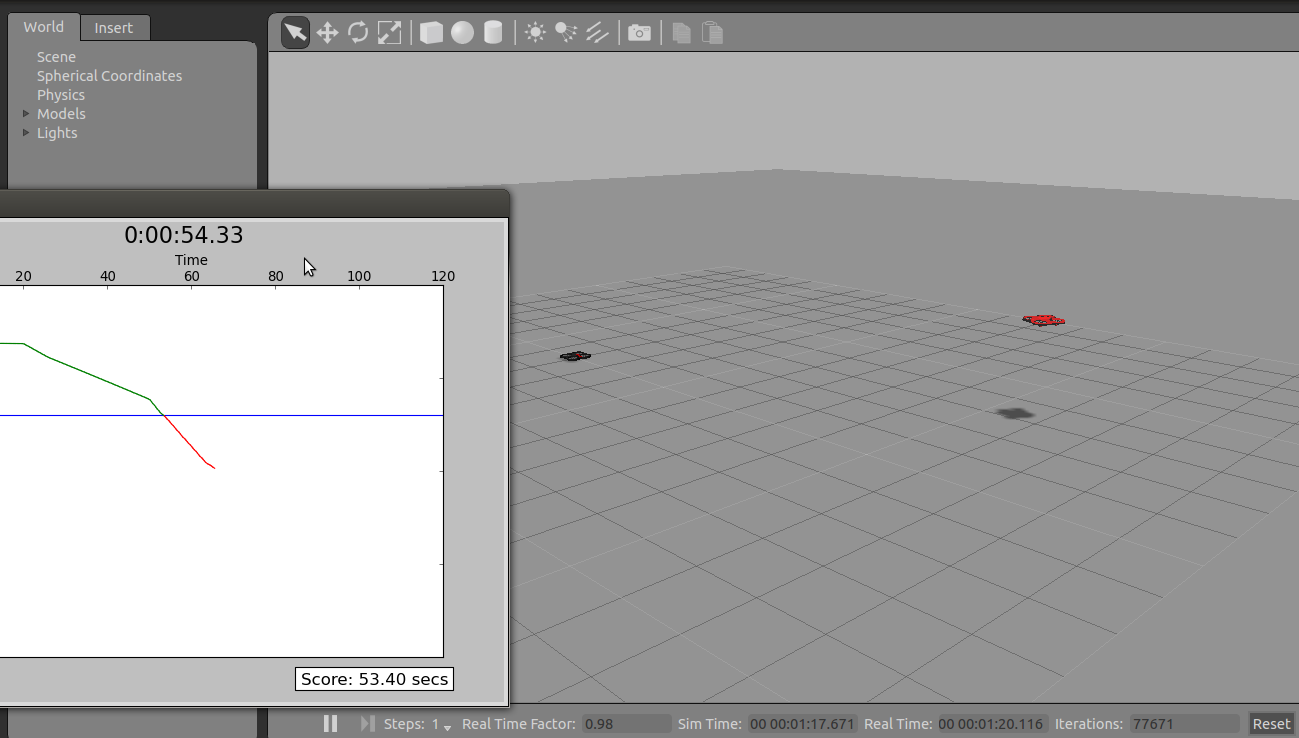
\includegraphics[width=0.7\textwidth]{gatoraton.png}
	\caption{Robot ArDrone en Gazebo persiguiendo a otro ArDrone dentro de una práctica.}
	\label{fig:gatoraton}
\end{figure}
	
	\item \textit{Control visual: sigue líneas}. En esta práctica el alumno debe conseguir que un robot Kobuki (\textit{Figura \ref{fig:kobuki}}) siga la línea roja de un circuito en el menor tiempo posible. El estudiante debe realizar los filtros de percepción necesarios para que el robot siga la línea roja y los movimientos del robot para mantenerse en la trayectoria adecuada.
	
	Esta práctica sirve para enseñar técnicas de percepción visual, de control reactivo, control basado en casos y de controladores PID.

\begin{figure}[h]
	\centering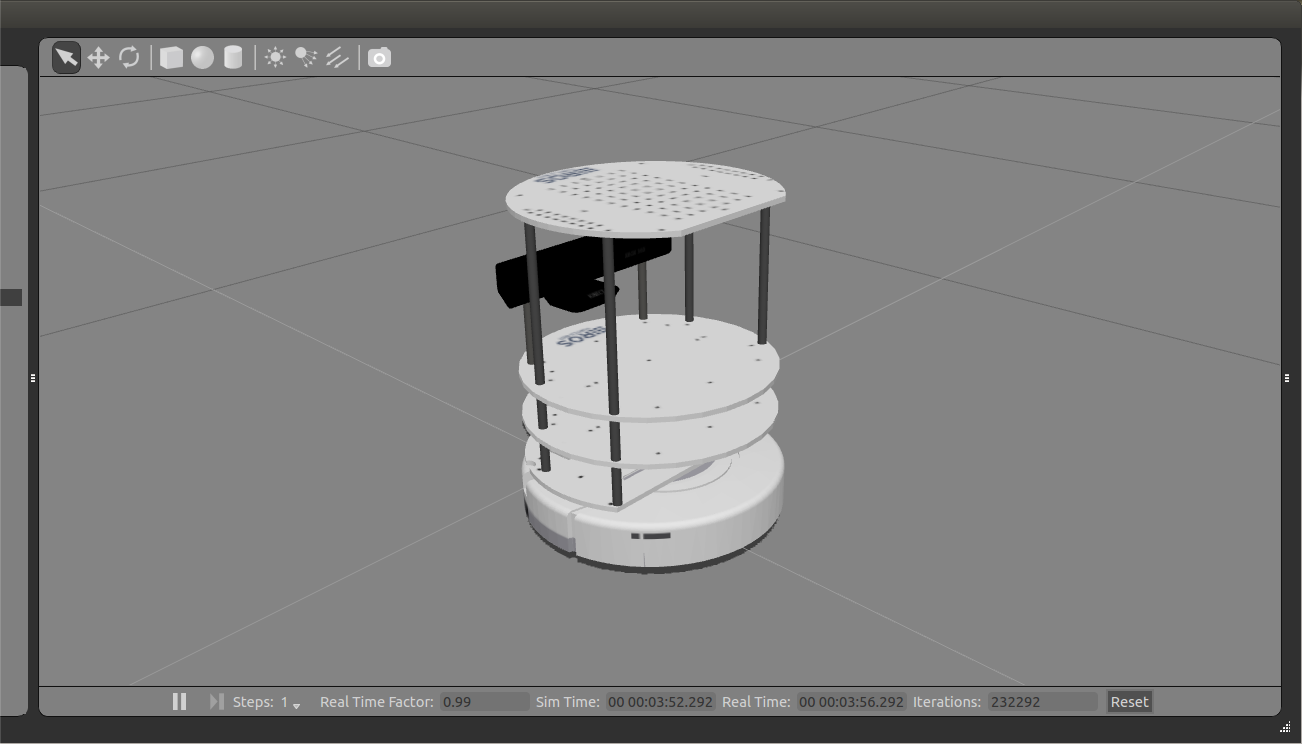
\includegraphics[width=0.4\textwidth]{turtlebot_simulado.png}
	\caption{Robot kobuki en Gazebo.}
	\label{fig:kobuki}
\end{figure}
	
	\item \textit{Fórmula 1: nacegación local}. En esta práctica el alumno debe programar un coche de Fórmula 1 (\textit{Figura \ref{fig:f1}}) para que complete una vuelta a un circuito de carreras esquivando los obstáculos que se encuentre en el camino. El robot cuenta con sensores de odometría, GPS y un sensor láser, y la interfaz de movimiento admite órdenes simples como velocidad de avanze o de giro.
	
	Para el desarrollo de esta practica se abordan algoritmos de navegación local como
	VFF (virtual force field) o campos virtuales, además de técnicas de percepción visual, de control reactivo o controladores PID.
	
\begin{figure}[h]
	\centering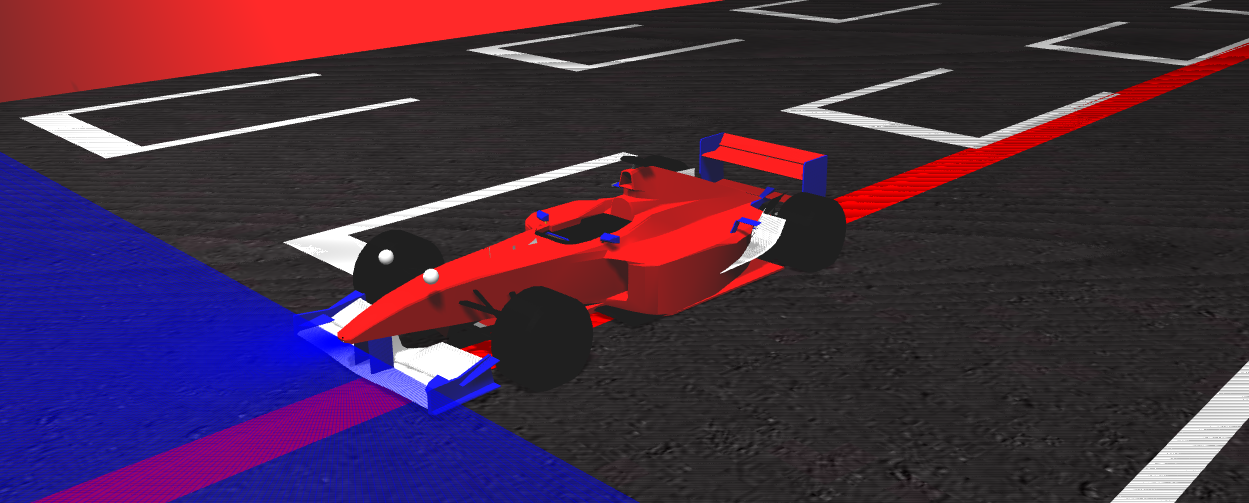
\includegraphics[width=0.4\textwidth]{f1.png}
	\caption{Robot de Fórmula 1 en un circuito en Gazebo.}
	\label{fig:f1}
\end{figure}
	
	\item \textit{TeleTaxi: navegación global}. En esta práctica el alumno debe conseguir que un coche vaya de un punto a otro cualquiera de una ciudad (\textit{Figura \ref{fig:teletaxi}}). El coche, taxi, tiene un sensor GPS y una interfaz como la del Fórmula 1. El alumno debe programar un algoritmo de navegación para que alcance la posición objetivo en un mapa conocido.
	
	En esta práctica se abordan, además de los elementos de control reactivo, algoritmos de planificación de caminos como Gradient Path Planning. En esta práctica no se necesitan elementos de percepción visual, ya que el taxi se guiará usando el GPS.

\begin{figure}[h]
	\centering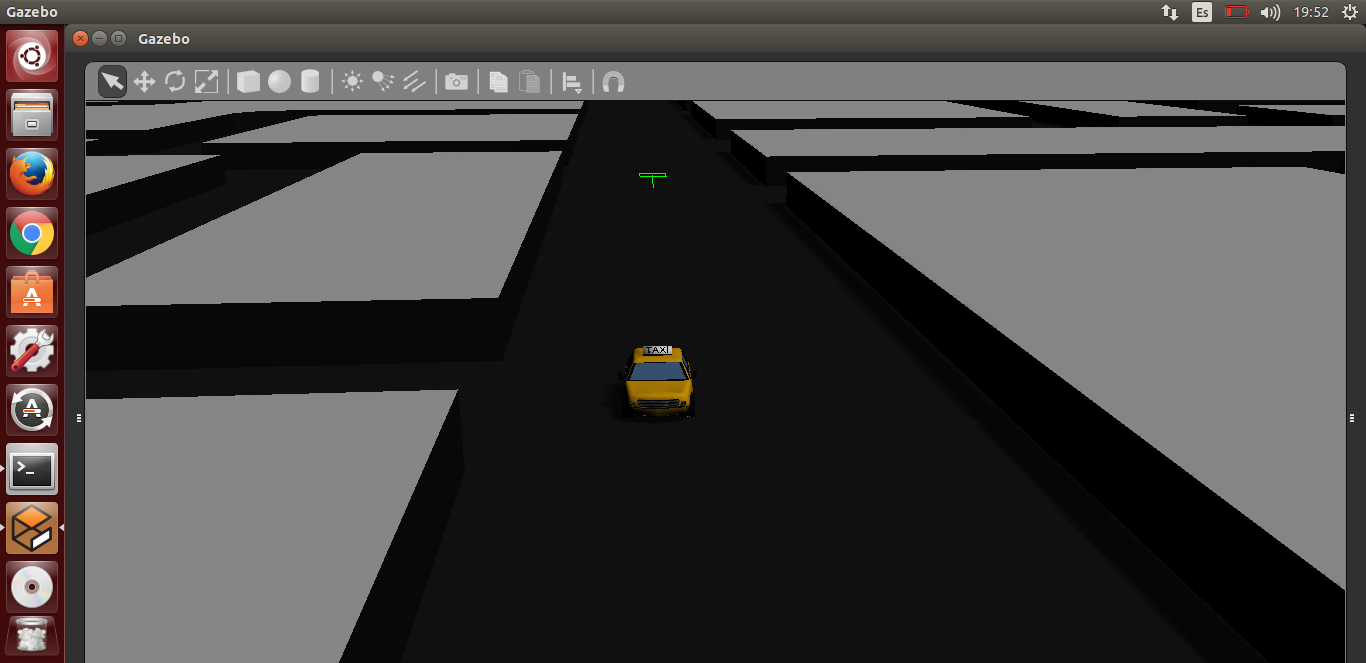
\includegraphics[width=0.6\textwidth]{teletaxi-city2.png}
	\caption{Robot taxi en una ciudad en Gazebo.}
	\label{fig:teletaxi}
\end{figure}
	
	\item \textit{Visión: reconstrucción 3D}. En esta práctica el alumno debe conseguir que un robot Pioneer (\textit{Figura \ref{fig:mundo3D}}) reproduzca en 3D los elementos que se le presentan. Este robot está equipado con un par estéreo de cámaras. Para conseguir su objetivo, el alumno debe programar un algoritmo de reconstrucción 3D clásico de tres pasos: detección de puntos de interés en las dos imágenes, emparejamiento de píxeles homólogos entre ambas, y triangulación espacial para calcular el punto tridimensional que origina cada pareja de píxeles homólogos.
	
	En esta práctica no se necesita que el robot se mueva, pero sí tiene una alta carga visual, pro lo que se abordarán técnicas de procesado de imagen y de percepción visual.
	
\begin{figure}[h]
	\centering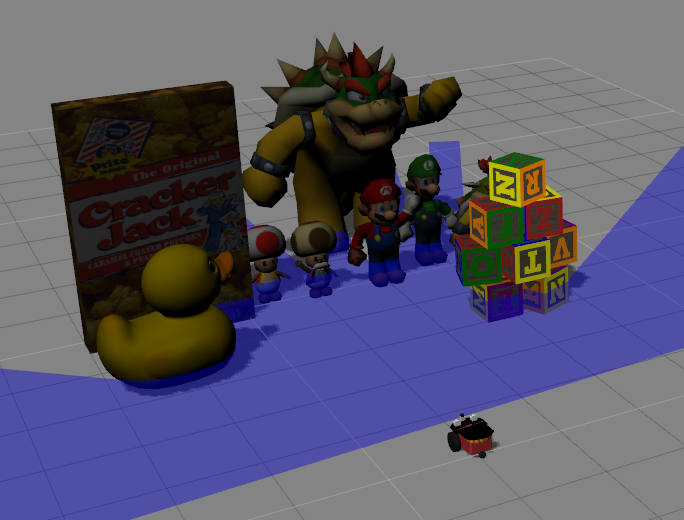
\includegraphics[width=0.5\textwidth]{mundo3D.png}
	\caption{Robot Pioneer en Gazebo frente al conjunto de objetos a escanear.}
	\label{fig:mundo3D}
\end{figure}

\end{itemize}

Nuestro objetivo con este trabajo es aumentar las posibilidades de esta plataforma, creando nuevos escenarios que aporten valor y funcionalidades nuevas a las prácticas ya existentes o desarrollando nuevas herramientas que permitan añadir prácticas más variadas a la colección.

En los siguientes capítulos cubriremos todos los elementos necesarios para lograr este objetivo. En el segundo capítulo abordaremos los objetivos marcados para este proyecto, así como los requisitos necesarios para cumplirlos y la metodología que usaremos. En el tercer capítulo expondremos los elementos usados como infraestructura, las herramientas que nos permitirán completar nuestra tarea. En el cuarto y quinto capítulo veremos las soluciones a las que hemos llegado para alcanzar los objetivos planteados, y en el sexto las conclusiones obtenidas de la realización de este proyecto, así como los futuros pasos a seguir.














meter cosas de metodologia EN EL CAPITULO 2




\chapter{Plataforma de Desarrollo}
\label{ch:PlataformaDesarrollo}

%breve introducción de la sección

\section{Blender}
\label{sec:plat_blender}

Blender\cite{blender} es un software libre y gratuito de creación en 3D. Está diseñado para realizar tareas como modelado, iluminación, renderizado, animación y creación de gráficos tridimensionales, edición de vídeo y escultura y pintura digital. En Blender, además, se pueden desarrollar vídeo juegos ya que posee un motor de juegos interno. Actualmente es compatible con todas las versiones de Windows, Mac OS X, GNU/Linux (Incluyendo Android), Solaris, FreeBSD e IRIX. Su interfaz utiliza OpenGL\footnote{\url{https://www.opengl.org/}} (\textit{Open Graphics Library}) para proporcionar una experiencia consistente y de calidad.

Blender fue liberado al mundo bajo los términos de la Licencia Pública General de GNU v2 (GPL)\footnote{\url{https://www.gnu.org/licenses/old-licenses/gpl-2.0.html}}, y su desarrollo continúa conducido por un equipo de voluntarios procedentes de diversas partes del mundo y liderados por el creador de Blender, Ton Roosendaal. 

Se eligió este programa para realizar la edición 3D de mundos para Gazebo frente a alternativas como 3DSMax, Maya o XSI por diversos motivos: es más ligero que sus competidores; posee más herramientas de escultura 3D; la comunidad es muy activa y hay gran cantidad de información, tutoriales y soluciones disponibles; y es de distribución comercial libre y gratuita. 


\section{Simulador Gazebo}
\label{sec:plat_gazebo}

Gazebo\cite{gazebo} es un simulador 3D de robots para interiores y exteriores, con un motor de físicas y cinemáticas muy potente. Dispone de un conjunto de plugins que facilita la integración con ROS, lo cual agiliza el desarrollo de código y permite la simulación de algoritmos antes de implementarlos en el robot físico, lo cual se puede lograr sin realizar apenas cambios en el código. Además está mantenido por una comunidad activa y la OSRF\footnote{\url{http://www.osrfoundation.org/}} (\textit{Open Source Robotics Foundation}), la cual también da soporte a ROS, y fué elegido para realizar el DARPA Robotics Challenge\footnote{\url{http://www.theroboticschallenge.org/}} entre 2012 y 2015.

Cabe destacar que Gazebo se compone principalmente de un cliente y un servidor. El servidor es el encargado de realizar los calculos y la generación de los datos de los sensores, y puede ser usado sin necesidad de una interfaz gráfica, por ejemplo en un servidor remoto. El cliente proporciona una interfaz grágica basada en QT que incluye la visualización de la simulación y una serie de controles de multitud de propiedades. Esta configuración permite lanzar multiples clientes sobre un servidor, consiguiendo multiples interfaces de la misma simulación

\section{JdeRobot}
\label{sec:plat_jderobot}

JdeRobot\cite{jderobot} es una suite de desarrollo de software de robótica, domótica y sistemas de visión computerizados cuya última versión, la 5.5, es la usada en este proyecto y permite la integración con ROS Kinetic. Proporciona un entorno distribuido donde las aplicaciones se forman mediante una colección de componentes asíncronos. Estos componentes utilizan interfaces ICE\footnote{\url{http://www.zeroc.com/}} para comunicarse, lo que permite lanzarlos desde distintos equipos y que estén escritos en diferentes lenguajes, como C++, Python o Java.

JdeRobot simplifica el acceso a elementos de hardware, siendo tan simple com realizar una llamada a una función. También permite que los sensores o actuadores con los que se comunica sean reales o simulados, conectados mediante la red tanto dentro de la misma máquina como en una red local o de forma remota mediante internet. Actualmente se han desarrollado drivers para una multitud de dispositivos, como por ejemplo sensores RGB como Kinect o cámaras USB o IP, vehículos como Kobuki o Pioneer, drones como el ArDrone de Parrot, etc.

Es un software libre, licenciado como GPL y LGPL que se sirve de software como Gazebo, ROS, OpenGL, QT... que se usa tanto para docencia como para investigación en la URJC y ha formado parte del \textit{Google Summer of Code 2015}\footnote{\url{https://summerofcode.withgoogle.com/organizations/6493465572540416/}}, programa donde Google premia a los estudiantes al completar un proyecto de programación de software libre durante un verano.


\section{ROS}
\label{sec:plat_ros}

El Sistema Operativo de Robots, ROS\cite{ros} (\textit{Robot Operating System}) es un entorno de trabajo flexible donde desarrollar software para robots. Es una colección de herramientas y librerías que buscan simplificar la tarea de crear comportamientos robustos y complejos en una amplia variedad de plataformas robóticas. 

Desde mediados de la década de los 2000 se han realizado esfuerzos para aunar los entornos y herramientas existentes en sistemas de software dinámicos y flexibles para su uso en robots. Estos esfuerzos culminaron, gracias al interés y la ayuda de innumerables desarrolladores, en las ideas que forman el núcleo de ROS y sus paquetes de software fundamentales. Desde entonces se ha expandido su uso bajo la licencia de software libre BSD\footnote{\url{https://es.wikipedia.org/wiki/Licencia_BSD}} y se ha convertido en una plataforma muy usada en la comunidad de investigadores.

Desde el inicio ROS se desarrolló en multitud de instituciones para multitud de robots, permitiendo a una gran variedad de investigaciones tener éxito bajo esta plataforma. Sólo el núcleo de ROS se mantiene en los servidores centrales, cualquier desarrollador es libre de crear, desarrollar y compartir sus propias ideas y proyectos de forma que, si así lo desea, estén disponibles para toda la comunidad desde sus propios repositorios. De esta forma se consigue mantener un ecosistema formado por decenas de miles de usuarios a nivel global, desde proyectos como hobby hasta sistemas industriales automatizados.

ROS se diseñó para ser modular y fragmentado, de modo que los usuarios pueden usar sólo las partes que necesiten. En bajo nivel ofrece una interfaz de comunicación por mensajes que permite ahorrar tiempo manejando los detalles de la comunicación entre nodos mediante un mecanismo anónimo de publicación/subscripción de mensajes estructurados. Este sistema fuerza al usuario a implementar interfaces limpias entre los nodos del sistema, mejorando la encapsulación y promoviendo la reutilización de código.

Adicionalmente ROS proporciona librerías y herramientas para agilizar el trabajo de sus usuarios. Dado el caracter colaborativo y comunitario del proyecto, se han unificado una gran variedad de formatos mensajes estándar que cubren la mayoría de las necesidades básicas en robótica, tales como posiciones, transformaciones, vectores, sensores como cámaras o lasers, datos de navegación como caminos o mapas, etc. 

Un problema común que aborda ROS es la descripción de un robot de forma que sea comprensible para un ordenador, consiguiendo un Formato Unificado de Descripción del Robot o URDF (\textit{Unified Robot Description Format}). Consiste en un fichero XML en que se describen las propiedades físicas del robot, partiendo del cual el robot se puede utilizar con librerías, simuladores y planificadores de movimientos.

También proporciona herramientas de diagnóstico, estimación, localización, navegación, así como una colección de herramientas gráficas y de línea de comandos para facilitar el desarrollo y la depuración. Las herramientas de línea de comandos permiten la utilización de ROS desde cualquier terminal, incluso con conexión remota. Las herramientas gráficas incluyen rviz y rqt, muy potentes tanto para planificar como para desarrollar proyectos en ROS.

Para entender mejor cómo funciona ROS podemos pensar en un sistema de grafos en el que situamos los siguientes elementos:

\begin{itemize}
	\item Nodos: Son las partes de código que se ejecutan. Escritos en C++ o Python permiten realizar tareas en el robot, subscribirse y publicar en topics o proporcionar y usar servicios. De esta manera se facilita el diseño modular de los proyectos.

	\item Topics: Son las vías de comunicación usadas por los nodos. Cada topic utiliza un único tipo de mensaje, de esta manera un nodo puede utilizar varios topics para comunicarse.

	\item Mensajes: Son los datos estructurados que se envían entre topics. En ROS existen varios tipos definidos para los mensajes más utilizados, pero se pueden definir nuevos tipos de mensajes de acuerdo con las necesidades particulares de cada proyecto

	\item Servicios: A diferencia de los topics, son vías de comunicación síncronas entre nodos compuestas por dos mensajes: uno de petición y otro de respuesta. De esta forma  el nodo que envía la petición espera hasta recibir la respuesta.
\end{itemize}

\subsection{MoveIt!}
\label{subsec:plat_moveit}

MoveIt!\cite{moveit}  es un software de código abierto para ROS (Robot Operating System) que es el estado de la técnica de software para la manipulación móvil. De hecho, podríamos afirmar que se está convirtiendo en un estándar de facto en el campo de la robótica móvil, ya que hoy en día más de 65 robots utilizan este software.

Incluye diversas utilidades que aceleran el trabajo con brazos robóticos, y sigue la filosofía de ROS de reutilización de código. Este software permite llevar a cabo tareas de planificación de trayectorias complejas, percepción 3D, cálculos cinemáticos, control de colisión, control y navegación de forma sencilla, accediendo por la API o mediante las herramientas de la consola.


\subsection{rviz}
\label{subsec:plat_rviz}

Rviz\cite{rviz} es una herramienta de visualización en 3D llamada que posibilita que  prácticamente cualquier plataforma robótica pueda ser representada en imagen 3D, respondiendo en tiempo real a lo que le ocurre en el mundo real. Se puede usar para mostrar lecturas de sensores y obtener información de estado de ROS.

Usado en conjunto con MoveIt! permite mostrar el brazo en su estado actual, la colocación del brazo en una posición objetivo, y la visualización del camino pensado por MoveIt! y del movimiento real del brazo siguiendo dicho camino.

\subsection{rqt}
\label{subsec:plat_rqt}

Rqt\cite{rqt} es un software de ROS que implementa varias herramientas de GUI (\textit{Graphical User Interface}) en forma de plugins, permitiendo cargarlas unificadas como una ventana en la pantalla facilitando trabajo al usuario. Simplemente con un comando en la consola, \textit{rqt} muestra una ventana donde elegir cualqier plugin disponible en el sistema en ese momento.

Contiene una herramienta que ha resultado muy útil para la realización de este proyecto: rqt\_graph. Al introducir en la consola \textit{rosrun rqt\_graph rqt\_graph} crea un grafo dinámico que muestra qué nodos y qué topics etán activos es ese momento y cuál es su relación. Al situar el ratón encima de cada elemento marcará con un código de color cuál es el elemento activo, de qué tipo es y cual es su relación con los demás elementos del grafo.


\section{ARIAC}
\label{sec:plat_ariac}

ARIAC\cite{ariac} (\textit{Agile Robotics for Industrial Automation Competition}) es una competición pionera cuyo objetivo es probar la agilidad de los sistemas robóticos industriales. Realizada por primera vez en Junio de 2017, nace de un esfuerzo conjunto entre la Conferencia de Automatización en Ciencia e Ingeniería del IEEE o CASE (\textit{Conference on Automation Science and Engineering}) y el NIST (\textit{National Institute of Standards and Technology}). Se sirve de Gazebo como plataforma de simulación y de un conjunto propio de modelos, plugins y scripts para simular un brazo robótico en un entorno dinámico, todo ello elaborado con la ayuda de la OSRF (\textit{Open Source Robotics Foundation}). Tiene el objetivo de aumentar la productividad y la autonomía de los robots industriales, entendiendo como agilidad la cosecución de manera automática de identificación de fallos y recuperación de los mismos, automatización para disminuir la reprogramación ante cambios en la producción, interacción con el entorno incluso en áreas no previstas inicialmente, y la capacidad de \textit{plug and play}, es decir, de introducir robots de otros fabricantes sin la necesidad de reprogramarlos.

En este proyecto nos servimos del entorno y del propio brazo robótico para desarrollar nuestros propios plugins para entender y controlar el brazo por medio de ROS.





\chapter{Circuito de carreras de Fórmula 1}
\label{ch:circuitocarreras}

Una vez explicado el contexto, los objetivos y las herramientas usadas en el proyecto, en este capítulo vamos ver en detalle la construcción de un mundo para Gazebo que se pueda usar en las prácticas de JdeRobot-Academy que emplean coches de carreras, en concreto el circuito de Fórmula 1 de Mónaco.

\section{Prácticas con circuito en JdeRobot-Academy}
\label{sec:circarr_practicas}

Las prácticas del entorno JdeRobot-Academy están diseñadas de forma que tanto el mundo como el robot están correctamente montados y configurados, y la aplicación que controla al robot está parcialmente completa. El alumno no necesita realizar modificaciones al mundo simulado o al robot, pero debe completar el código de la aplicación para realizar las tareas propuestas en la práctica. En la figura \ref{fig:graficof1} podemos ver la relación entre los componentes software de estas prácticas, así como el espacio destinado al trabajo del alumno. Marcado con una flecha roja esta Gazebo, para señalar las partes modificadas con este Trabajo Fin de Grado. No cambiamos nada del coche ni de la aplicación docente, sí cambiamos el mundo de Gazebo para lograr que la misma práctica se situe en otro escenario.

\begin{figure}[h]
	\centering
	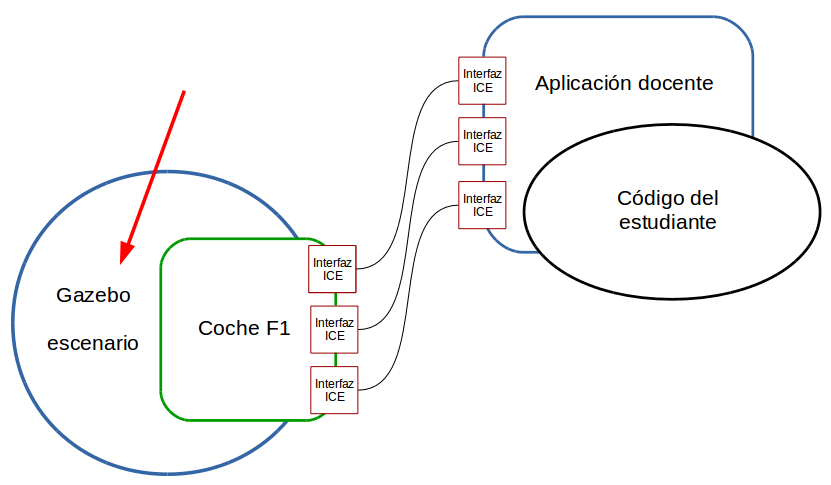
\includegraphics[width=0.8\textwidth]{graficof1.png}
	\caption{Esquema de los componentes de las prácticas con Fórmula 1.} \label{fig:graficof1}
\end{figure}

Actualmente el entorno JdeRobot-Academy presenta dos prácticas basadas en circuitos de Fórmula 1:
\begin{itemize}
	\item Práctica de navegación local autónoma: En esta práctica el Fórmula 1 dispone de unos sensores que le permiten detectar obstáculos. En la figura \ref{fig:vff} podemos apreciar el funcionamiento del sensor comparando la información que recibe con la vista real de la simulación. En esta práctica el alumno ha de rellenar el código con elementos de percepción, que le permitan identificar los obstáculos, y con algoritmos de navegación local como el VFF (visual force field), logrando dar vueltas al circuito esquivando los obstáculo presentes.
	
	\item Práctica de sigue-línea: En esta práctica el Fórmula 1 dispone de una cámara con la que capta imágenes del circuito. En este caso el circuito dispone de una línea roja en el suelo, y el coche ha de seguir esa línea para completar las vueltas. En esta práctica el alumno ha de programar el código con algoritmos de procesamiento de imagen, como filtros de color o de formas, y con elementos de control como controladores PID para que el robot siga la línea.
\end{itemize}
	
\begin{figure}[h]
	\centering
	\subfigure[Vista del simulador.]{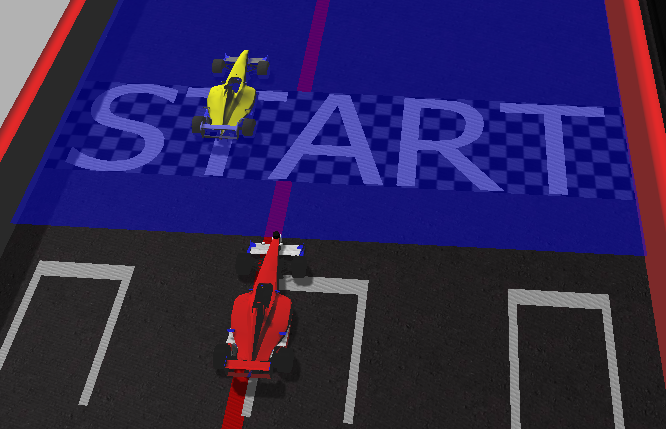
\includegraphics[width=0.47\textwidth]{vff-gazebo.png}}
	\subfigure[vista del sensor.]{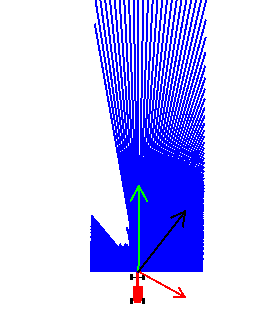
\includegraphics[width=0.25\textwidth]{vff-gui.png}}
	\caption[Vistas de la práctica de navegación local del F1.]{Vistas de la realización de la práctica, tanto lo que muestra Gazebo (a) como una representación de lo que recibe el sensor (b).} \label{fig:vff}
\end{figure}

Nuestro objetivo es reconstruir el circuito de Mónaco de forma que se pueda utilizar en ambas prácticas, creando para ello mundos de Gazebo que se acoplen al esquema de funcionamiento de estas prácticas, como muestra la flecha de la figura \ref{fig:graficof1}.

\section{Manejo de Blender}
\label{sec:circarr_manejodeblender}

En esta sección vamos a explicar cómo se utiliza este potente programa de creación, renderizado y animación de gráficos tridimensionales. El uso de este tipo de programas es, a priori, de los más difíciles, ya que trabajar sobre un mundo tridimensional en una pantalla de ordenador, desplazando un ratón sobre una mesa en dos dimensiones, exige un esfuerzo de abstracción considerable.

Es por ello que en los primeros pasos de esta sección nos dedicaremos a presentar la interfaz del programa y exponer la inmensa cantidad de opciones y herramientas de que dispone, centrándonos en aquellas que han resultado relevantes para la consecución de los objetivos marcados.


\subsection{Interfaz}
\label{subsec:circarr_interfaz}

Como se verá, la interfaz de Blender no sigue el patrón típico de los programas a los que estamos habituados, como editores de texto y hojas de cálculo o entornos de desarrollo de software, por lo que resulta fácil desorientarse al principio.

La interfaz de usuario de Blender está compuesta por 4 ventanas por defecto, como se pueden diferenciar en la figura \ref{fig:interfazblender01}. Cada ventana tiene una cabecera con las herramientas adecuadas para trabajar sobre
dicha ventana y, a su vez, cada herramienta está dotada de sus correspondientes pestañas para una completa edición. Esta disposición facilita y agiliza el uso apropiado del programa. A su vez, cada cabecera de cada ventana tiene el botón Tipo de Editor, mediante el cual se puede cambiar el tipo de ventana que se muestra, por lo que se puede personalizar el aspecto para agilizar el trabajo.

\begin{figure}[ht]
	\centering
	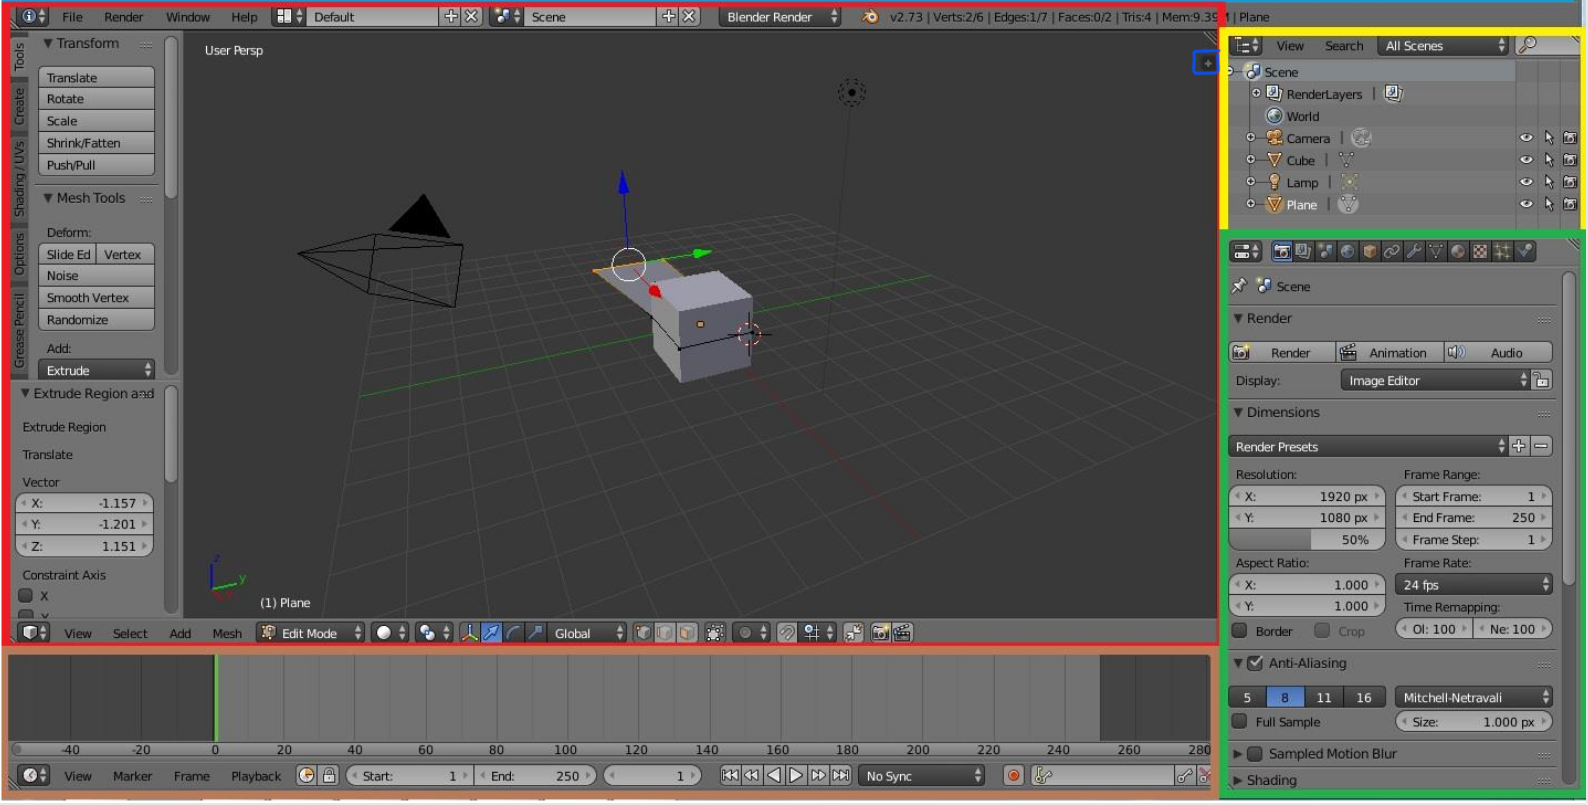
\includegraphics[width=0.9\textwidth]{InterfazBlender01.png}
	\caption{Interfaz de Blender.} \label{fig:interfazblender01}
\end{figure}


En primer lugar tenemos la ventana de Vista 3D, bordeada en color Rojo. En esta ventana se visualiza todo el trabajo y los cambios que se realizan con el programa. En esta ventana podemos observar los siguientes objetos y menús:

\begin{itemize}
	\item Manipuladores de Transformaciones en 3D (\textit{Figura \ref{fig:interfazblender03}}): Muestra de manera visual información de las transformaciones a realizar. Cada objeto puede ser transformado de tres maneras: traslación (G), rotación (R) y escalado (S). Utilizando la combinación Ctrl+Space,	o bien haciendo clic en el icono del sistema de coordenadas, se puede mostrar y ocultar el manipulador. 
	\begin{figure}[h]
		\centering
		
\includegraphics[width=0.30\textwidth]{InterfazBlender03.png}
		\caption{Detalle de Manipuladores de transformaciones en 3D.} \label{fig:interfazblender03}
	\end{figure}
	
	
	\item Cursor 3D (\textit{Figura \ref{fig:interfazblender04}}): El cursor 3D es una herramienta muy útil y se utiliza para una variedad de cosas como representar el lugar donde se añadirán nuevos objetos o representar el punto de pivote para una rotación. Sin embargo, es muy engorroso a la hora de trabajar ya que es muy fácil moverlo accidentalmente y al necesitar usarlo se pierde bastante tiempo reubicándolo.
	\begin{figure}[h]
		\centering
		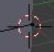
\includegraphics[width=0.12\textwidth]{InterfazBlender04.png}
		\caption{Detalle del cursor de Blender.} \label{fig:interfazblender04}
	\end{figure}

	\item Cubo: Al iniciar Blender, por defecto, aparece un cubo situado en el centro de la ventana 3D. Es uno de los elementos básicos que se pueden insertar y la mayoría de las veces basta este simple cubo para comenzar a trabajar.
	
	\item Luz (de tipo lámpara): Al iniciar Blender, por defecto, también aparecerá una Luz de tipo lámpara que estará en algún sitio cerca del centro de la escena. Es posible crear otras fuentes de luz, como un sol en el cenit de la escena o una luz direccional que ilumine todos los objetos. En cualquier caso, aunque en los diferentes modos de edición no sea necesario, a la hora de renderizar la escena para visualizar el resultado del trabajo es necesaria alguna fuente de luz, si no, aparecerá una escena llena de siluetas.
	
	\item Cámara: Al iniciar Blender, por defecto, aparecerá una cámara que estará en algún sitio por el centro de la ventana 3D y, probablemente, enfocando al cubo. En la figura \ref{fig:interfazblender01} es esa especie de pirámide de vértices negros a la izquierda del cubo. A la hora de renderizar es necesaria una cámara.
	
	\item Objeto seleccionado actualmente: Este campo, situado en la parte inferior izquierda de la escena, al lado del eje de coordenadas, muestra el  nombre del objeto seleccionado actualmente.
	
	\item Modo Edición: Este botón, en forma de desplegable, se encuentra a la izquierda de los botones de manipuladores de transformaciones 3D. Da acceso a un modo de edición para manipular la geometría del objeto. Al activarse aparecen disponibles tres botones de opciones, justo a la derecha de los botones de manipuladores de transformaciones 3D. Nos permiten cambiar entre la selección y edificación de los vértices, de las aristas y de las caras del objeto. La posibilidad de cambiar entre estas opciones de selección es especialmente útil a la hora de dar forma a los objetos que componen el circuito.
	
	\item Vista de la escena: Este botón, en forma de desplegable, se encuentra a la derecha del botón de Modo Edición. Da acceso a un desplegable que permite elegir la vista de la escena 3D entre las posibles, como sólida, texturas, materiales, ”wireframe”, renderizada, etc. Nos permite ver los objetos de la escena con sólo las texturas, sólo los vértices, ya renderizado, etc, para poder trabajar más cómodo en según que condiciones y ver los resultados de aplicar texturas o del renderizado final.
	
\end{itemize}

Para realizar con comodidad el trabajo sobre cualquier tipo de elemento existen diferentes vistas disponibles, cada una con un atajo de teclado propio, en concreto del teclado numérico. De esta forma para el “1” el programa proporciona una vista frontal de la escena; con el número “3” se obtiene una vista derecha; etc. Una de las más cómodas para realizar el trabajo es la que le corresponde al número “7” ya que se trata de una vista cenital, que una vez superpuesto el plano del circuito facilitan la tarea de trazar el recorrido. Por último, con la tecla “5” podemos cambiar la vista de Perspectiva a Ortográfica. La vista Perspectiva es la más similar a la realidad, dando profundidad a la escena y sensación de lejanía y proximidad de los objetos. La vista Ortográfica es más artificial, pues es como una proyección de la anterior, pero es útil en determinadas situaciones para no alterar las proporciones o manejar con fluidez objetos que quedarían tapados de otra forma.

Esta ventana posee un botón de propiedades propio marcado en color Azul en la parte superior derecha, el cual despliega la ventana de propiedades (\textit{Figura \ref{fig:interfazblender02}}). Esta ventana muestra las propiedades del objeto seleccionado y resulta muy útil a la hora de añadir nuevos bloques o realizar modificaciones de los ya existentes, pudiendo modificar la localización, rotación, escala, etc.

\begin{figure}[h]
	\centering
	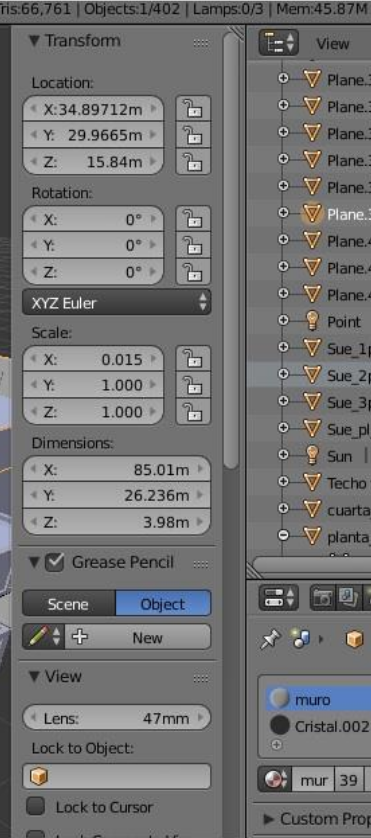
\includegraphics[width=0.4\textwidth]{InterfazBlender02.png}
	\caption{Ventana de propiedades.} \label{fig:interfazblender02}
\end{figure}

Debajo de la ventana de vista 3D, bordeada en marrón, se encuentra por defecto la ventana de Línea Temporal. Aquí se reflejan cronológicamente los bloques u objetos que se han añadido o modificado y es muy utilizada al trabajar con animaciones. En nuestro caso la hemos sustituido por otra que se adapta mejor a nuestras necesidades.

A continuación, bordeada en amarillo, se puede identificar la ventana de Objetos y Jerarquías, donde se pueden ver todos los datos que se utilizan en el trabajo. De esta forma se pueden controlar los diferentes bloques que se utilicen, las luces que se añaden a la escena, cámaras y toda clase de elementos disponibles en la escena. En esta ventana se pueden seleccionar directamente los elementos que se deseen independientemente, y realizar acciones sobre ellos como restringir o habilitar la visualización, selección o renderización de dicho elemento. Esto supone una gran ayuda cuando se superponen diferentes elementos en la ventana.

Debajo de ésta, marcada en color verde, se encuentra la ventana de Propiedades, en la cual se pueden editar las propiedades de los bloques, objetos, materiales, texturas etc. que se utilizan en el trabajo. Esto se consigue mediante los llamados botones de contexto, los cuales muestran un grupo de paneles con opciones diferentes para cada botón. Gracias a esta disposición se esconden multitud de herramientas muy usadas en un espacio reducido y cómodo. Algunas de las tareas que permiten llevar a cabo son: asignar el material o la textura deseada a los elementos creados o modificaciones para replicar, deformar, dividir o desdoblar elementos entre muchas otras opciones

\section{Creación de un circuito plano}
\label{sec:circarr_circuitoplano}

Una vez presentadas las opciones básicas de Blender y cómo desenvolverse entre ellas con un mínimo de soltura pasaremos a desarrollar el proceso de creación del circuito de Mónaco. En este proyecto comenzamos creando el trazado del circuito  sin elevaciones, para coger soltura en el manejo del programa y explorar las diferentes opciones antes de realizar tareas más complejas. 

Vamos a replicar en Blender los diferentes tramos y elementos del circuito como distintos objetos con textura, materiales, etc. Los juntaremos con un objeto plano compuesto que también tiene el mar para conseguir recrear el trazado y sus alrededores.

\begin{figure}[ht]
	\centering
	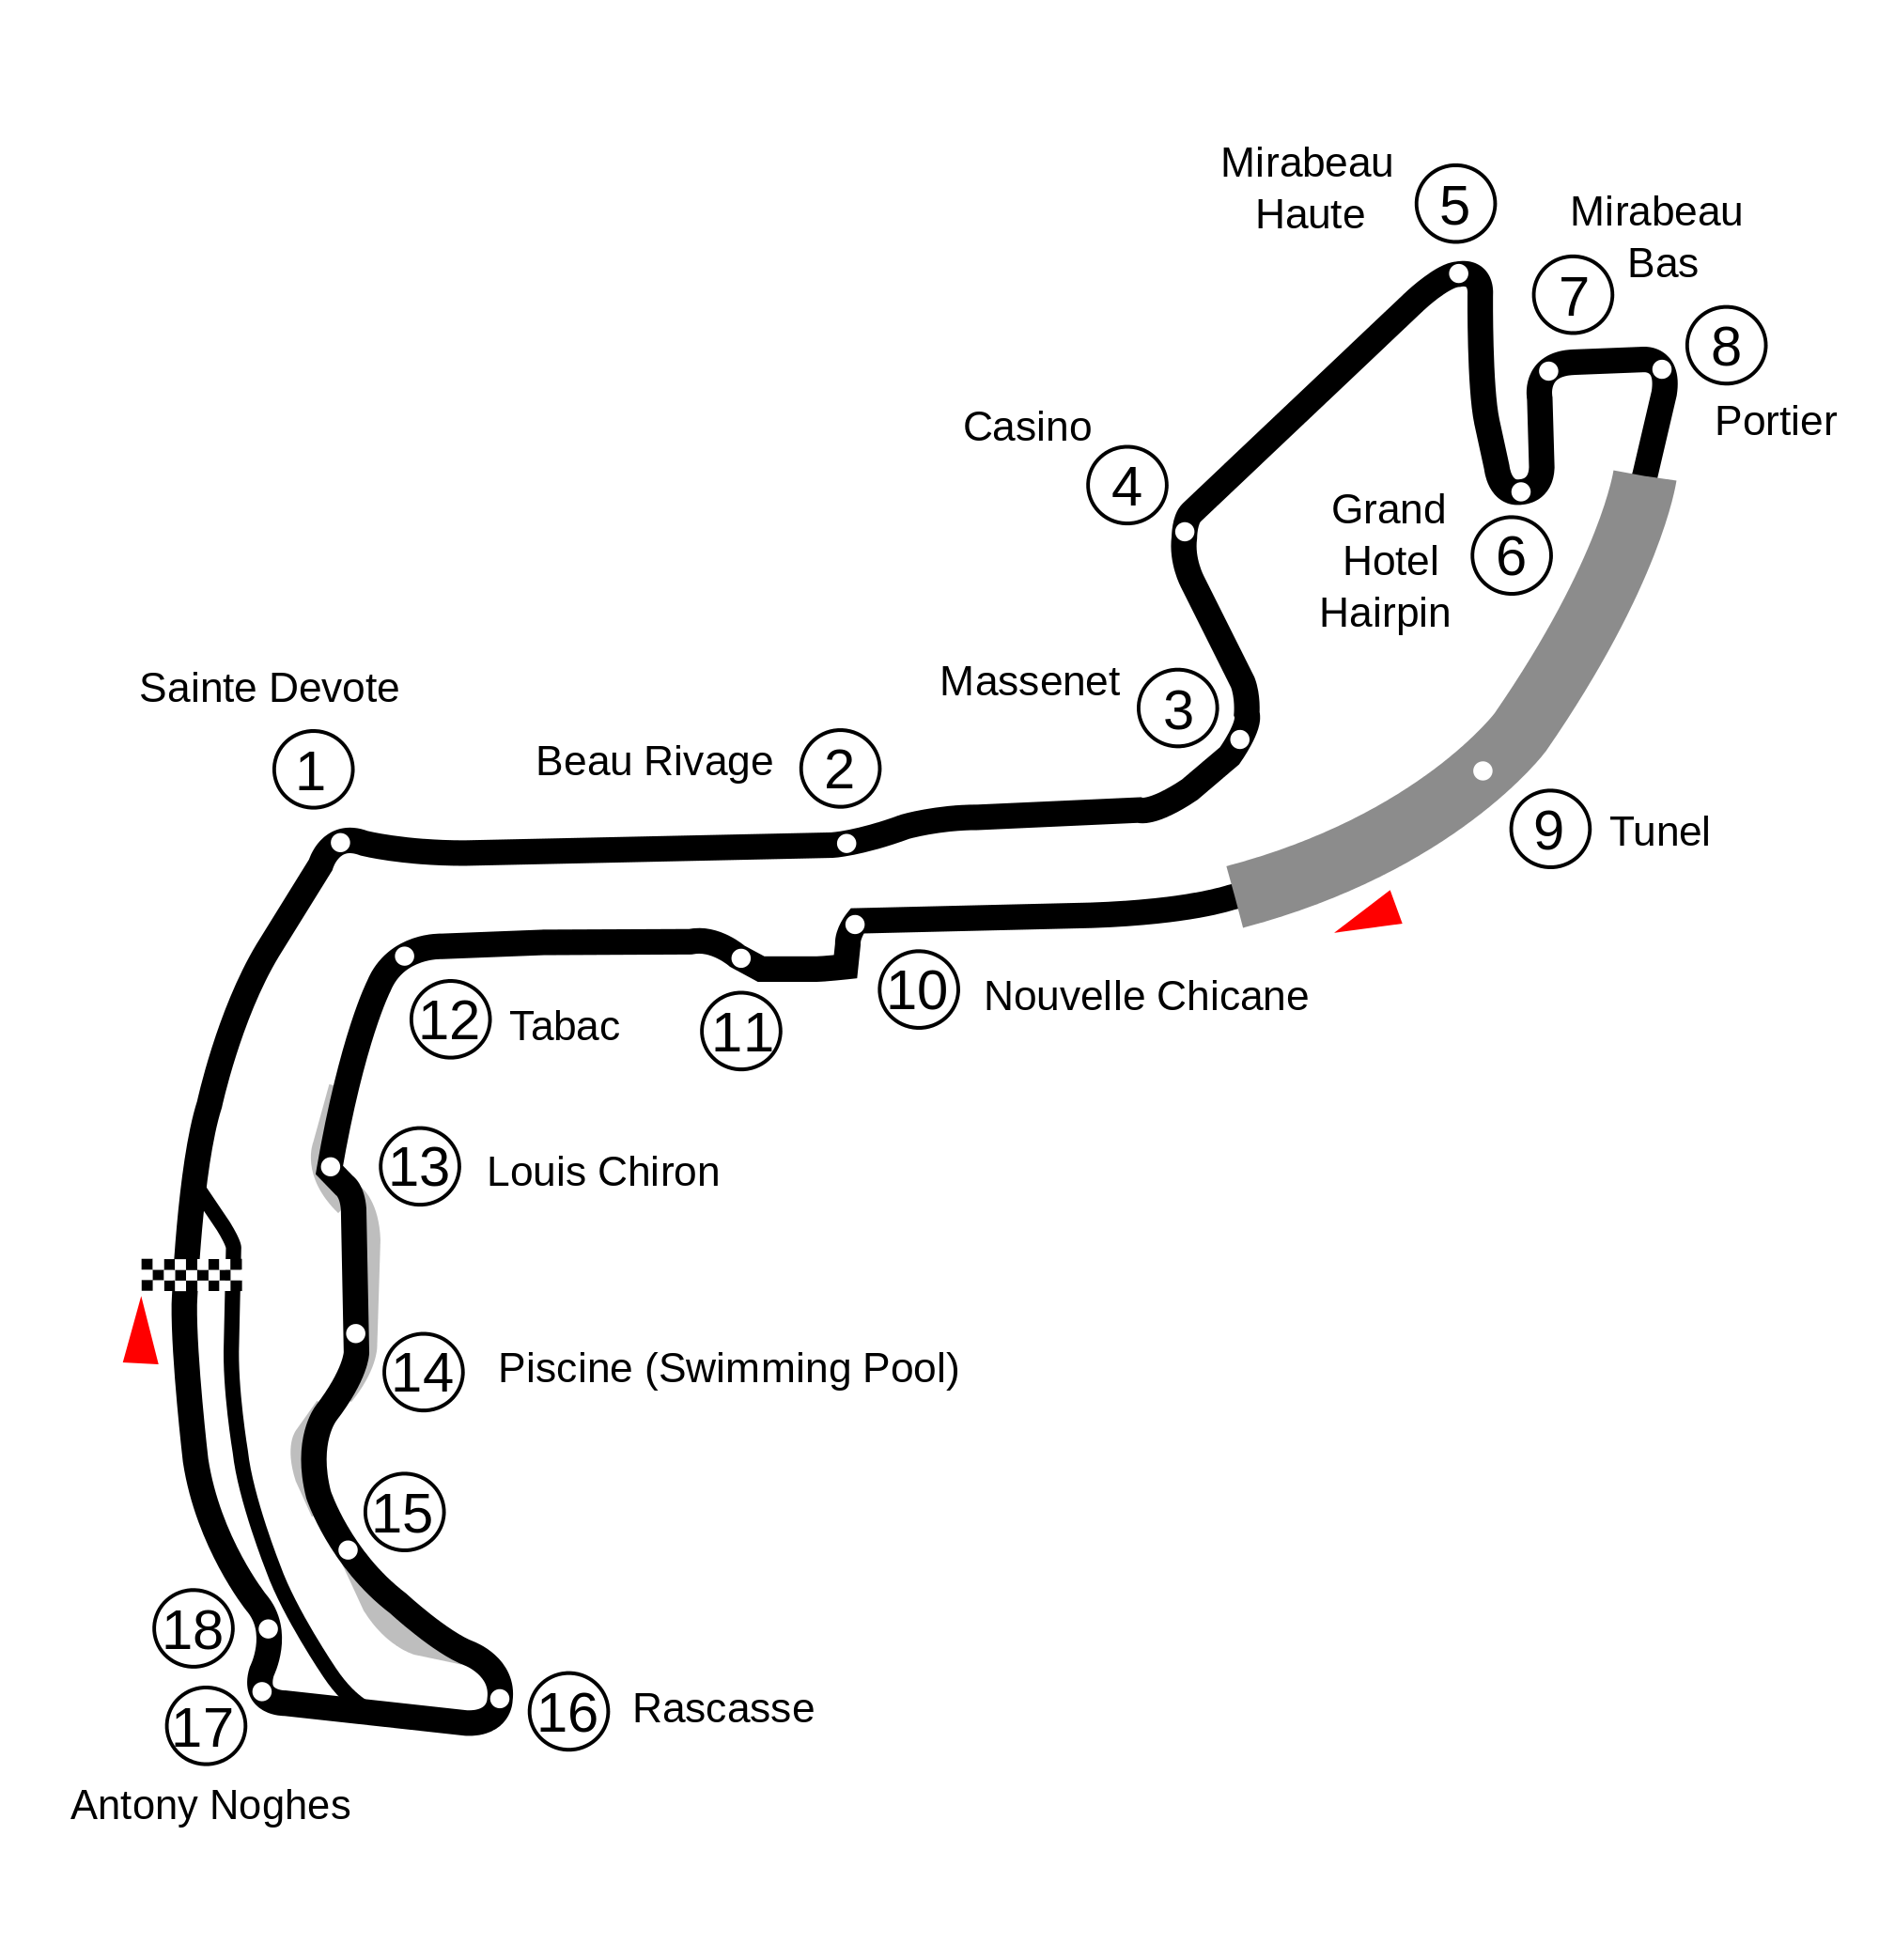
\includegraphics[width=0.5\textwidth]{CircuitoMonaco.png}
	\caption{Trazado del circuito de Mónaco usado como plantilla.} \label{fig:circuitomonaco}
\end{figure}

Comenzamos eliminando el cubo que aparece por defecto, desplegando la ventana de propiedades del menú principal y buscando el apartado de “Background Images”. Activamos la casilla y buscamos la imagen que deseamos poner de fondo, en este caso la imagen de la figura  \ref{fig:circuitomonaco}. Es el trazado real del circuito, visto desde arriba. Lo usaremos como plantilla creando curvas y tramos de carretera en Blender que se solapen con estas. Al hacer click en el botón “Add Image” podremos seleccionar la imagen que queremos ver de fondo, así como el eje en el que la queramos ver. Esta herramienta es especialmente útil ya que  nos permite ver una superposición de la imagen del trazado al usar la vista cenital, que corresponde con la tecla “7” del teclado numérico, pero en cualquier otro ángulo no se verá, con lo que facilita enormemente la tarea de escalado y modelado del circuito.

A continuación añadimos una curva “Bezier” (\textit{Figura \ref{fig:interfazblender05}}), hacemos esto desde el menú superior en \textit{Add}, \textit{Curve}, \textit{Bezier}. Esto creará un nuevo objeto, que podemos renombrar en la ventana de Objetos para facilitar el acceso y la selección posteriormente, cuando tengamos mas objetos en la escena. Este tipo de curvas, como se puede apreciar en la figura \ref{fig:interfazblender05}, son unas curvas com muchos elementos que nos permiten moldearlas a nuestro gusto. En cada extremo del tramo se componen de una recta con tres puntos. el central que establece el inicio del trazo de la curva, y los otros dos que establecen el giro de la curva y lo pronunciado que és. Cuanto más cerca estén del punto central más cerrado será el ángulo de giro, y cuanto más alejados más suave la curva descrita.

\begin{figure}[h]
	\centering
	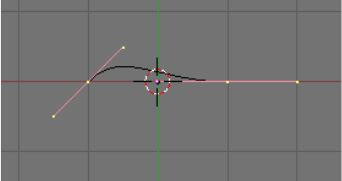
\includegraphics[width=0.5\textwidth]{InterfazBlender05.png}
	\caption{Detalle de curva Bezier.} \label{fig:interfazblender05}
\end{figure}

Al hacer click con el botón izquierdo del ratón mientras mantenemos la tecla Control pulsada añadimos un nuevo punto a la curva ya existente. De esta forma podemos ir añadiendo puntos y deformando la curva hasta que se superponga con la imagen del trazado. Así logramos una curva cerrada correspondiente al trazado sobre la cual situar los elementos que compondrán la carretera, como podemos apreciar en la Figura \ref{fig:monacotrazado} (\textit{La línea naranja es la curva Bezier que será el trazado}).

A continuación añadimos un plano haciendo \textit{Add}, \textit{Mesh}, \textit{Plane}, lo cual generará un cuadrado plano en el centro de la escena A continuación seleccionamos una arista y la extruimos (\textit{estiramos}) dos veces, una más corta y una más larga. hacemos lo mismo con la arista opuesta del cuadrado. Es importante realizar este paso ayudándonos de las flechas de colores (\textit{verde, rojo y azul}) que aparecen al seleccionar un objeto para mantener el conjunto en el mismo plano. Una vez realizado, extruimos los dos rectángulos más pequeños hacia arriba, consiguiendo crear la carretera, las vallas y una acera para el circuito, aunque de momento sólo aparecen en gris.

\begin{figure}[ht]
	\centering
	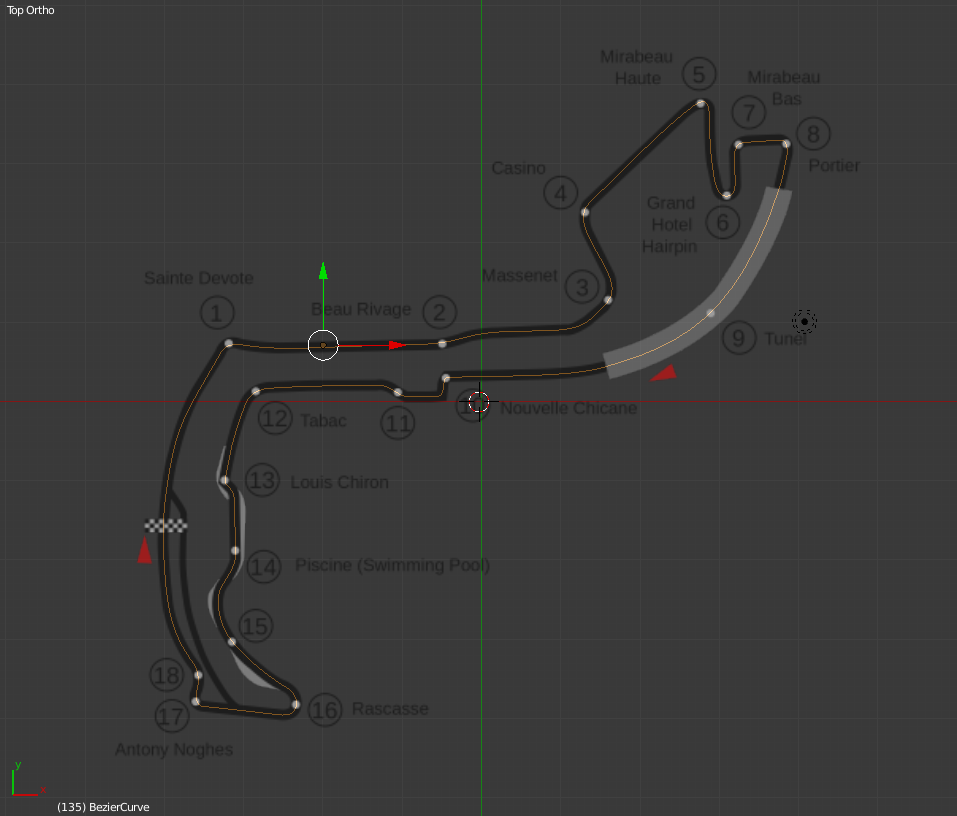
\includegraphics[width=0.85\textwidth]{MonacoTrazado.png}
	\caption{Trazado del circuito de Mónaco superpuesto a la plantilla.} \label{fig:monacotrazado}
\end{figure}

Para ayudarnos en la labor de texturizar objetos, editamos el tipo de ventana que es la de la parte inferior, el gráfico temporal, y lo sustituimos por un Editor de Imagen/UV, el cual posee herramientas avanzadas de manejo de imágenes para texturizado de superficies. De esta manera vamos cara por cara de nuestro objeto seleccionándola en la vista 3D, añadiendo una textura\footnote{Las imágenes usadas como texturas y materiales en este proyecto han sido obtenidas de manera gratuita de la página textures.com\cite{texturescom}} en el Editor UV, y observando los resultados en la vista 3D cambiando el modo de visualización a texturizado. La ventana del Editor de imagen nos sirve para redimensionar las texturas, girarlas, pintar encima de ellas, establecer qué zonas aparecen en la superficie seleccionada, y multitud de herramientas que hacen mucho más sencilla la edición de texturas. Una vez finalizado el paso de texturizar las caras del objeto obtenemos el segmento de la figura \ref{fig:monacosegmento}.

\begin{figure}[h]
	\centering
	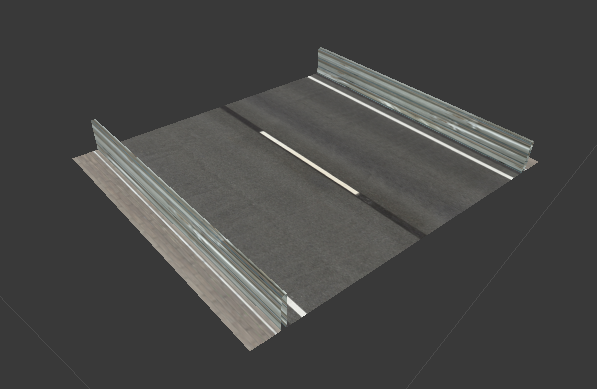
\includegraphics[width=0.5\textwidth]{MonacoSegmento.png}
	\caption{Segmento del circuito.} \label{fig:monacosegmento}
\end{figure}

Es muy importante crear un material para cada textura y asignarlo a las caras correspondientes, de otra manera no se aplicará la textura al renderizar y será como haber trabajado en vano. Esto se consigue mediante la ventana de propiedades y haciendo click en la pestaña de materiales. Es necesario crear un material nuevo, añadir como fuente la misma imagen que se ha usado como textura anteriormente, renombrar para no confundirlos más adelante, y asignarlo a la superficie correspondiente. Además, en la pestaña texturas, debemos repetir los pasos para crear la textura de la misma forma que el material. Necesitaremos además asignar cada textura al material correspondiente y cambiar el tipo de mapping a UV. Es una tarea laboriosa pero muy importante, ya que de no realizarse correctamente las texturas podrían no aplicarse y el objeto aparecería gris plano.

\begin{figure}[hb]
	\centering
	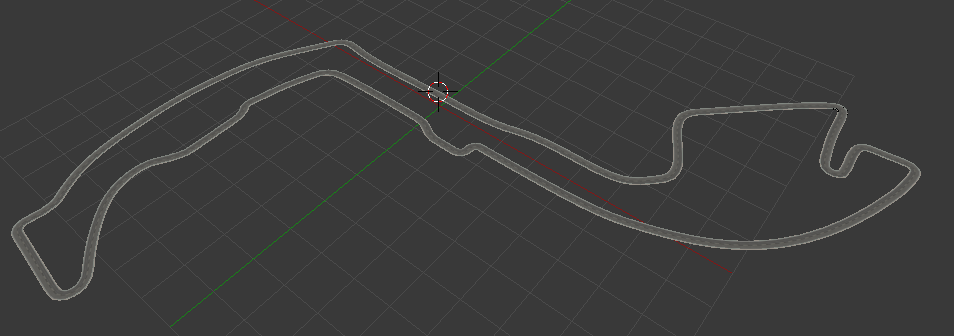
\includegraphics[width=1\textwidth]{MonacoTrazado1.png}
	\caption{Circuito (sólo el trazado).} \label{fig:monacotrazado1}
\end{figure}

Una vez realizados todos estos pasos seleccionamos el segmento del trazado creado y vamos a la ventana de propiedades y hacemos click en la pestaña de modificadores. Añadimos un nuevo modificador, un Array. Con esto conseguimos crear multitud de objetos iguales conectados entre sí, como si de un circuito de \textit{Scalextric} se tratase. Despues añadimos otro modificador, una curva en este caso, y elegimos como elemento modificante la curva Bezier que hemos creado anteriormente. De esta manera, jugando con el número de copias que realiza el array, conseguimos que el segmento creado se repita y deforme siguiendo el trazado de la curva, adquiriendo la forma del circuito deseado. Este método requiere de muchos retoques manuales, ya que en los vértices de las curvas cerradas el programa no puede calcular bien y solapa y deforma de manera incorrecta los vértices del segmento. Una vez realizados todos los retoques, así como la unión del primer y último segmento, obtenemos el objeto de la figura \ref{fig:monacotrazado1}.

Una vez obtenido el primer trazado completo necesitamos añadir un plano que servirá de fondo para el circuito. Para ello añadimos un nuevo objeto plano a la escena, lo aumentamos de tamaño hasta que se pueda situar el circuito en su interior y lo subdividimos en cuadrículas. Esto lo hacemos así para poder asignar texturas a cada cuadrícula independientemente y simular de manera más realista que este circuito se sitúa en un puerto, estando a la orilla del mar casi la mitad de su recorrido. Una vez realizada la división deformamos algunos vértices escondiéndolos debajo del trazado, necesitando así menos divisiones y aligerando la carga de procesamiento para la simulación del circuito. Una vez asignadas todas las texturas, repitiendo los pasos descritos para texturizar el segmento del circuito, obtenemos el circuito de Mónaco (\textit{Figura \ref{fig:monacoplano1}}), el cual podemos ver en detalle en la Figura \ref{fig:monacoplanovistas}.

\begin{figure}[t]
	\centering
	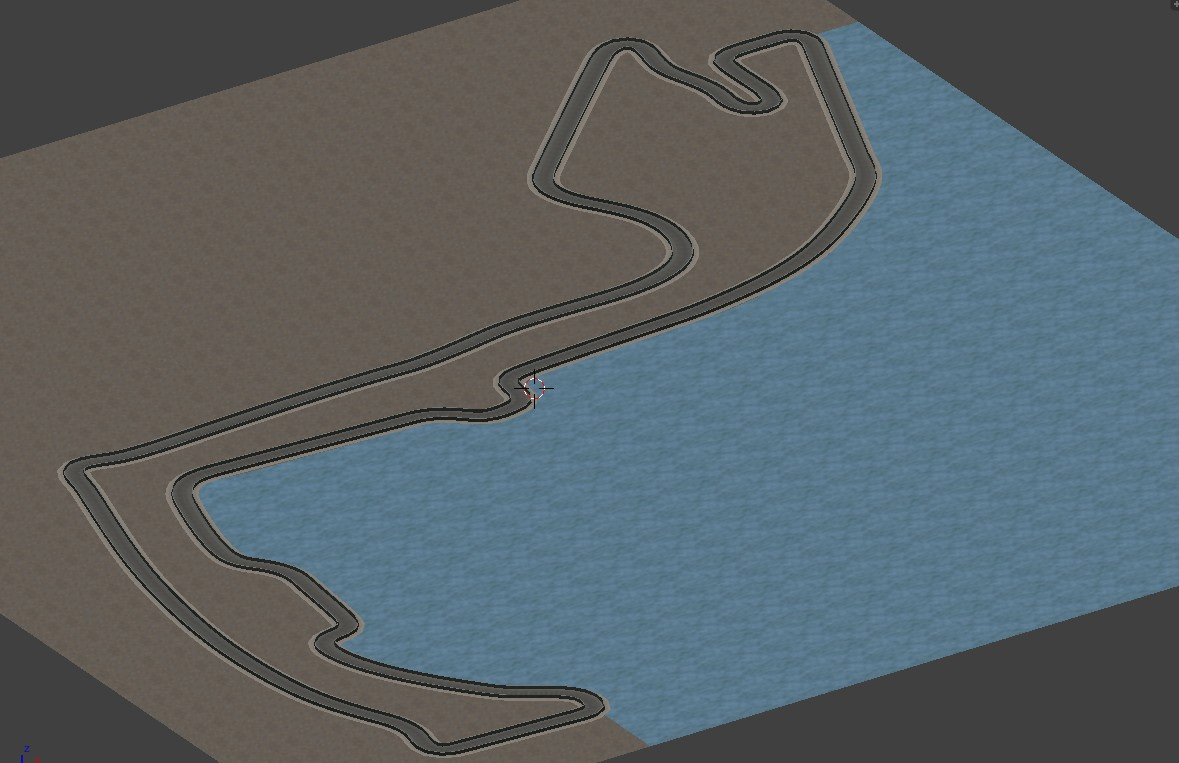
\includegraphics[width=0.7\textwidth]{MonacoPlano1.jpg}
	\caption{Circuito plano.} \label{fig:monacoplano1}
\end{figure}

\begin{figure}
	\centering
	\subfigure{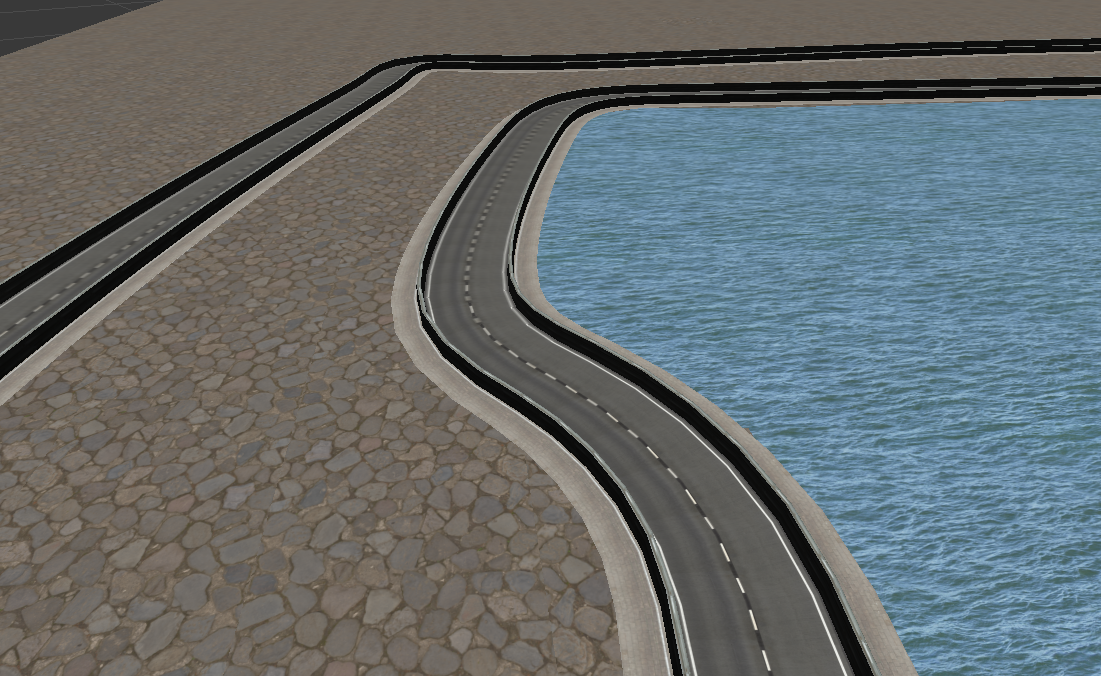
\includegraphics[width=0.47\textwidth]{MonacoPlano2.png}}\hspace{0.02\textwidth}	
	\subfigure{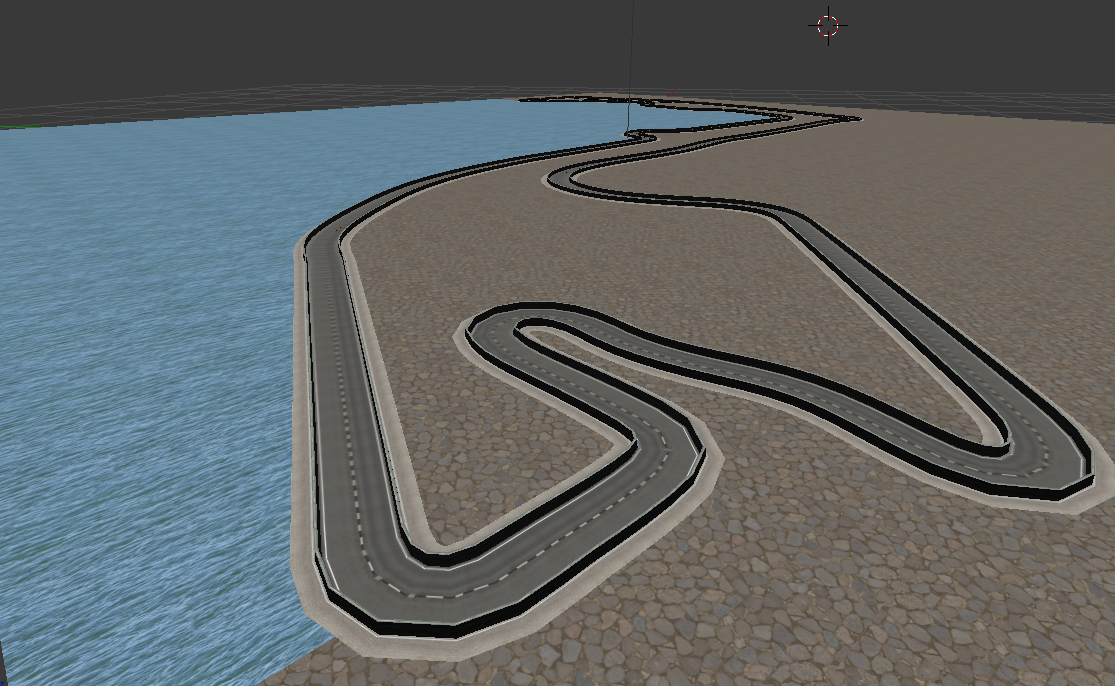
\includegraphics[width=0.47\textwidth]{MonacoPlano9.png}}\vspace{0.01\textwidth}
	\subfigure{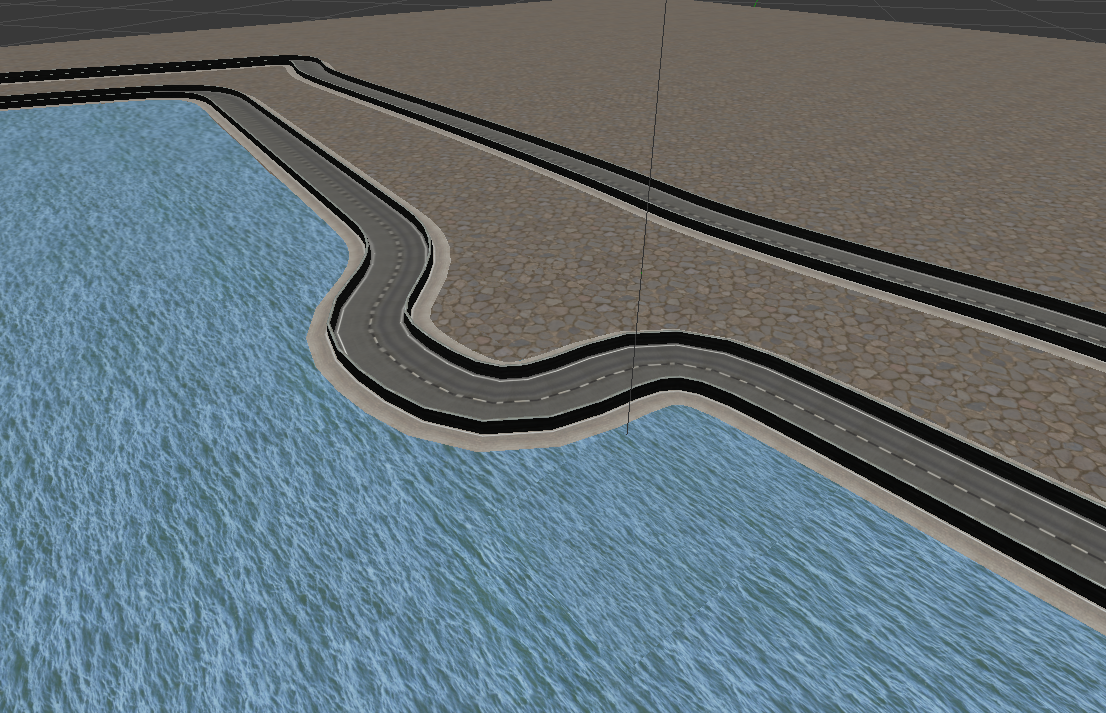
\includegraphics[width=0.47\textwidth]{MonacoPlano10.png}}\hspace{0.02\textwidth}
	\subfigure{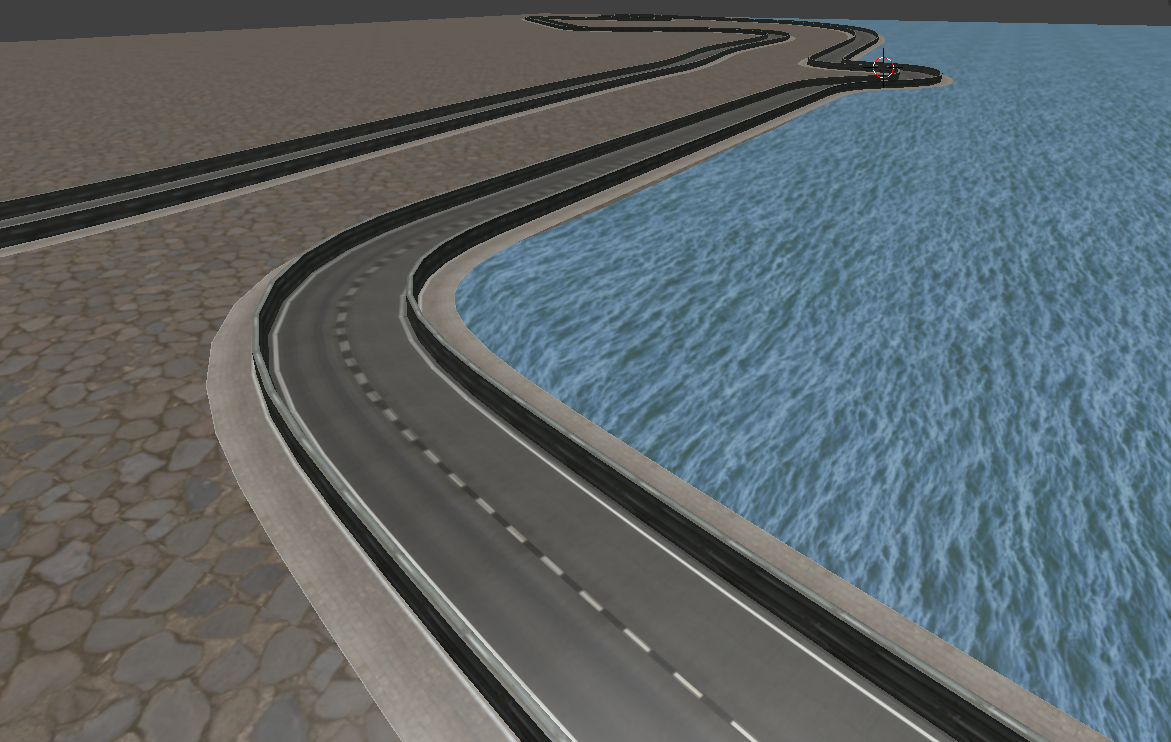
\includegraphics[width=0.47\textwidth]{MonacoPlano3.png}}
	\caption{Diferentes vistas del circuito de F1 de Mónaco plano.} \label{fig:monacoplanovistas}
\end{figure}


\section{Creación del circuito con elevaciones}
\label{sec:circarr_circuitoconelevaciones}

Una vez modelado el circuito plano pasamos a modelarlo ahora con elevaciones. Dada la dificultad de simplemente añadirlas al circuito ya creado, partimos de cero en la creación de este nuevo escenario. Puesto que ahora es mucho más relevante el fondo, comenzamos por esa parte. Eliminamos el cubo por defecto y añadimos un nuevo objeto, ésta vez una \textit{Mesh}, \textit{Grid}, que llamaremos rejilla. Es diferente del plano por que ya está subdividido, como una rejilla. Al crearlo, en la parte inferior izquierda de la ventana de vista 3D, aparecen una serie de propiedades únicas de este objeto que modificamos a nuestro gusto. En este caso el número de subdivisiones de la rejilla y el tamaño de ésta. Elegimos una cantidad moderada de divisiones ya que, aunque van a afectar visualmente a que las elevaciones no sean todo lo suaves que desearíamos, van a condicionar la carga de procesamiento del mundo en Gazebo, y queremos que sea todo lo ligera posible para poder realizar prácticas con múltiples objetos y vehículos sin que se vea comprometido el rendimiento.

Haciendo click en el botón de Modo Edición accedemos a otro modo, en este caso de Escultura. Una vez en este modo, en la parte superior izquierda de la ventana de vista 3D se despliega una multitud de herramientas y opciones para esculpir los objetos de la escena. Como lo que nos interesa es elevar la rejilla de forma que simule las alturas y elevaciones del circuito real de Mónaco, accedemos a la opción de bloqueo y seleccionamos los ejes x e y, con lo que sólo modificaremos la altura del plano sobre el que proyectaremos el trazado. Modificando las opciones del pincel hasta dejarlo a nuestro gusto comenzamos a esculpir la rejilla. Usando la misma imagen de antes como plantilla de fondo y fotos reales del circuito esculpimos un prototipo de lo que serán las elevaciones, que más tarde retocaremos para ajustarnos mejor a las peculiaridades del trazado. También nos serviremos de otro tipo de pincel para alisar las rugosidades creadas al modelar de forma más basta y así suavizar el terreno para acomodar mejor al circuito.

\begin{figure}[t]
	\centering
	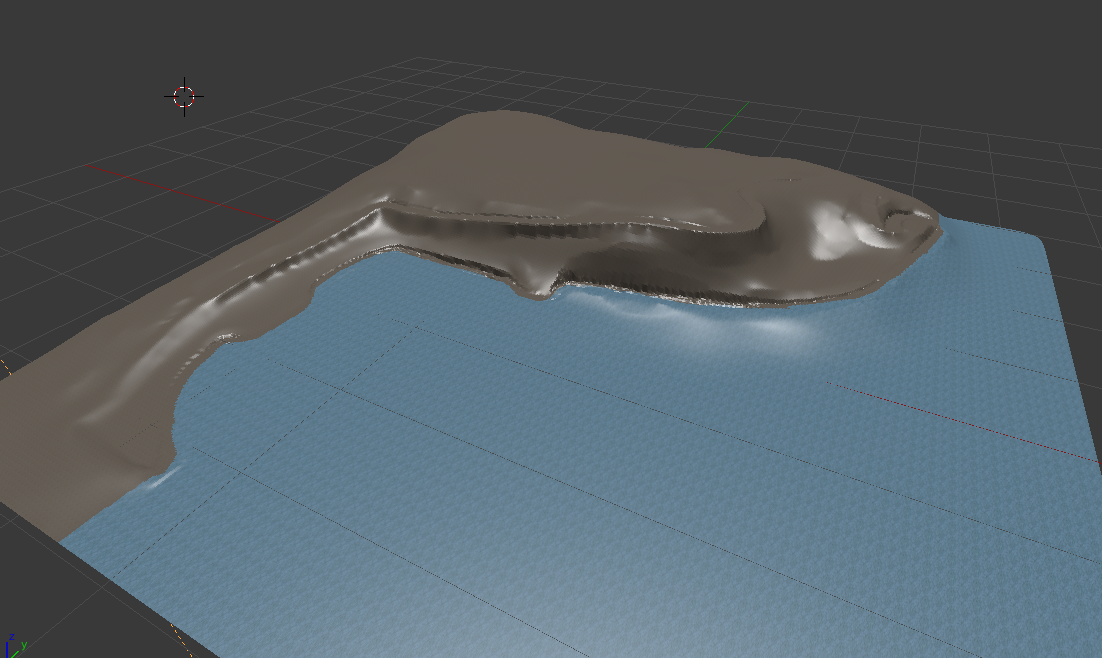
\includegraphics[width=0.75\textwidth]{MonacoElev00.png}
	\caption{Fondo para el circuito con elevaciones.} \label{fig:monacoelev00}
\end{figure}

A continuación creamos de nuevo, siguiendo los mismos pasos, la curva Bezier que servirá de trazado. Creamos ahora un plano, que pintamos de un color llamativo, y extendemos a lo largo de la curva bezier, consiguiendo un trazado de referencia para acabar de dar los últimos detalles a la rejilla. Tanto a la curva como a este plano le aplicamos como modificador la rejilla, consiguiendo darles altura y pudiendo ver el recorrido real del circuito con las elevaciones modeladas. Ahora modelamos la rejilla teniendo en cuenta el recorrido del circuito y su situación a orillas del mar, por lo que tenemos mucho cuidado de mantener plana toda la parte baja y del mar y aplicamos las elevaciones en las demás partes. Una vez modelado texturizamos de forma análoga a como hicimos anteriormente. Una vez modelado y texturizado el plano, eliminamos el trazado de referencia y obtenemos el suelo sobre el que descansará el circuito (\textit{Figura \ref{fig:monacoelev00}}).

Ahora repetiremos todos los pasos de creación del trazado (creamos el segmento, lo texturizamos, lo extendemos a lo largo de la curva) y además le aplicamos la rejilla como modificador. Si hemos realizado bien el paso anterior con el trazado de referencia, el trazado final debería descansar sobre la caja realizada y acoplarse perfectamente al terreno, de no ser así retocamos nuevamente la rejilla con las herramientas de escultura. 

\begin{figure}[hb]
	\centering
	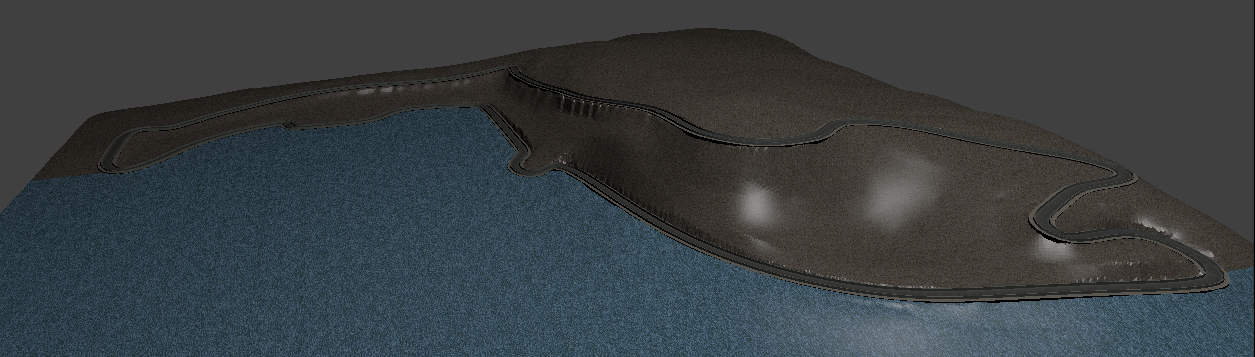
\includegraphics[width=1\textwidth]{MonacoElev05.png}
	\caption{Circuito con elevaciones.} \label{fig:monacoelev05}
\end{figure}

Una vez completado este paso podemos dar por finalizado el circuito (\textit{Figura \ref{fig:monacoelev05}}). En la Figura \ref{fig:monacoelevvistas} se pueden ver detalles del circuito donde se aprecian mejor las elevaciones del terreno.

\begin{figure}[h]
	\centering
	\subfigure{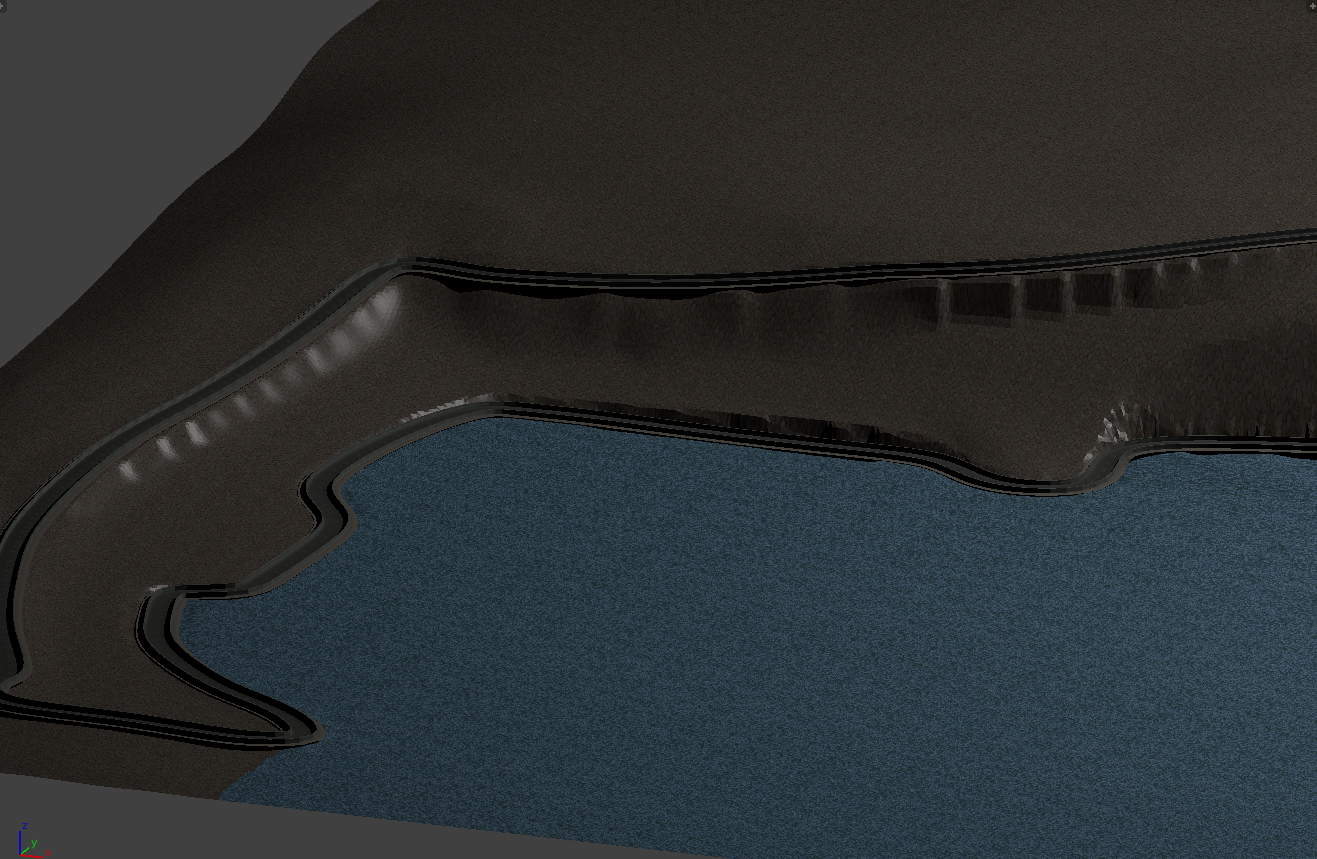
\includegraphics[width=0.495\textwidth]{MonacoElev01.png}}
	\subfigure{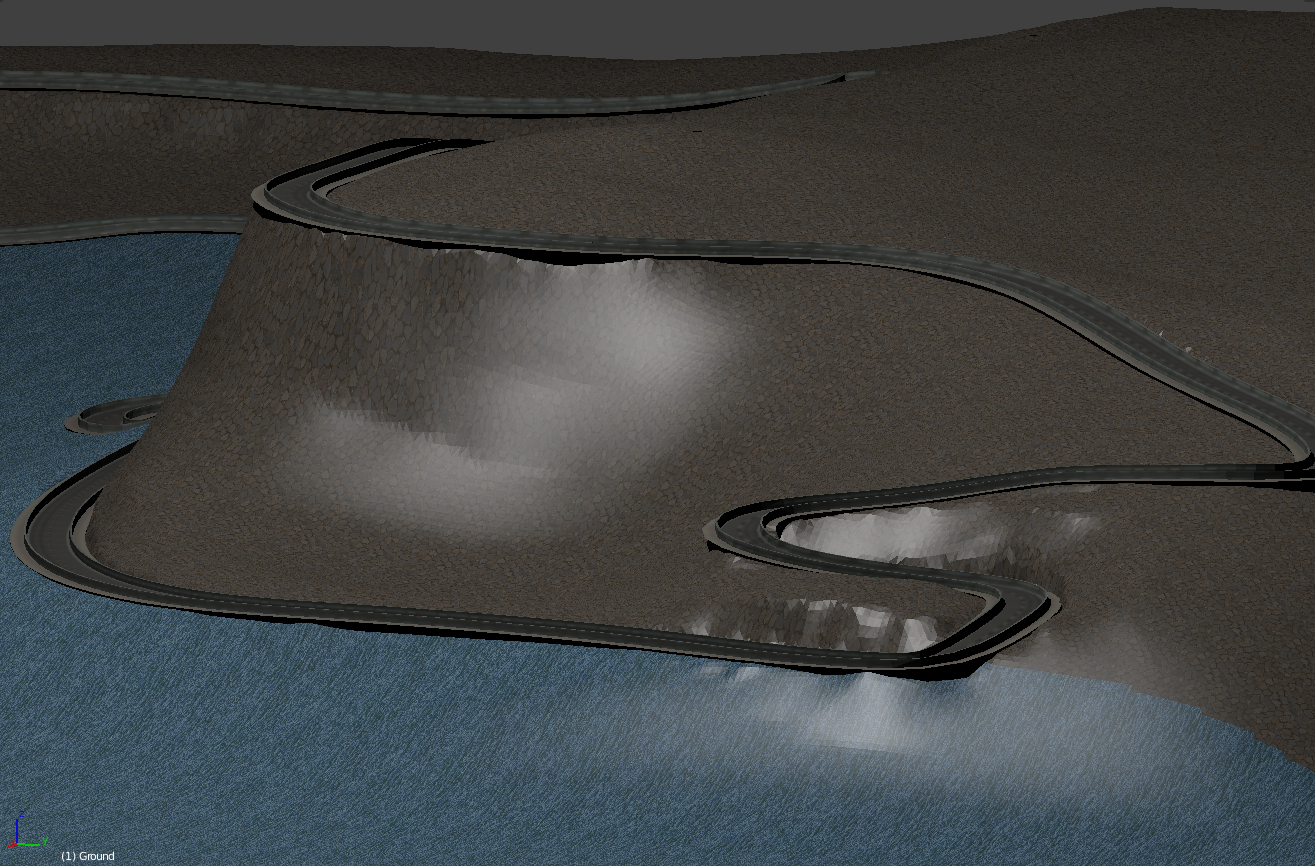
\includegraphics[width=0.495\textwidth]{MonacoElev02.png}}
	\subfigure{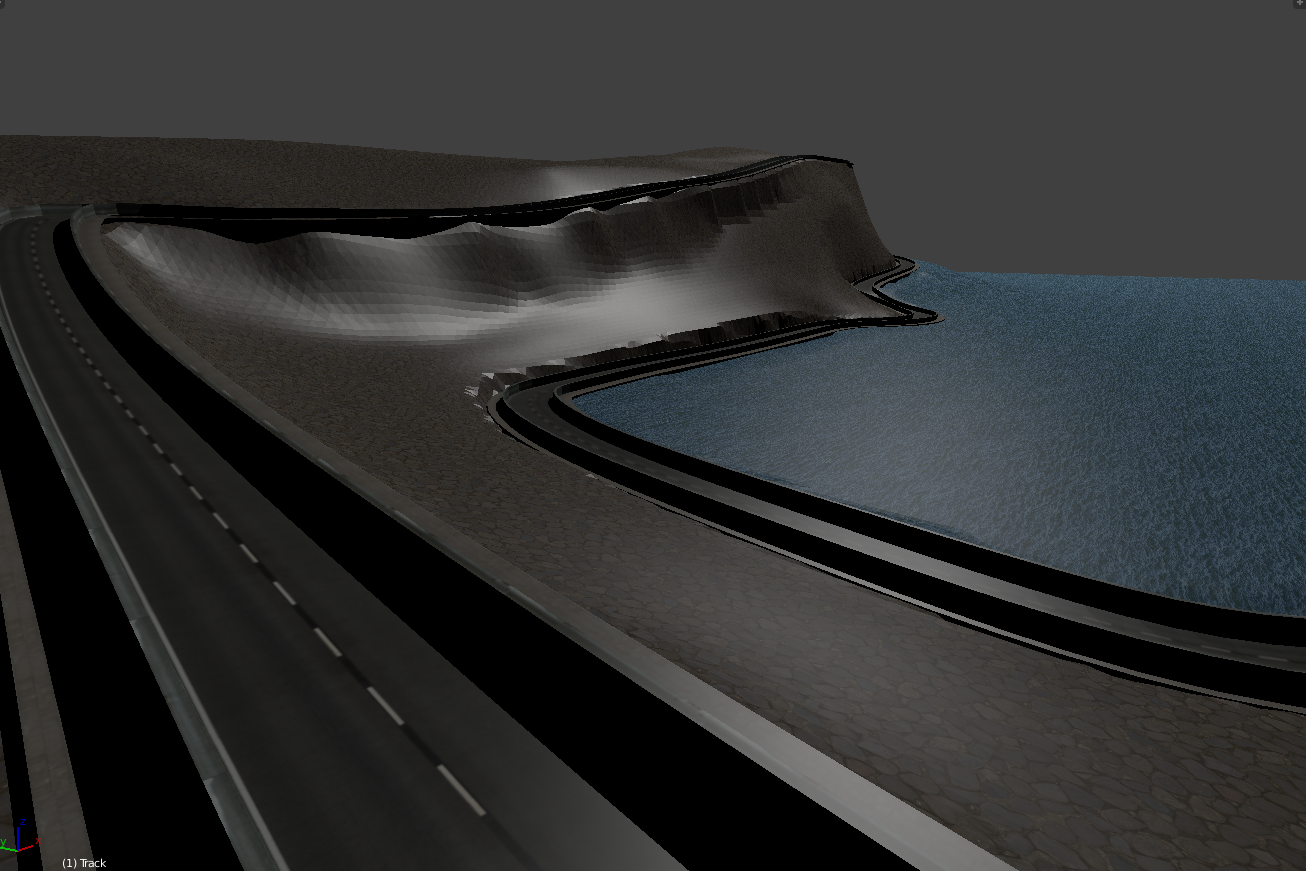
\includegraphics[width=0.495\textwidth]{MonacoElev03.png}}
	\subfigure{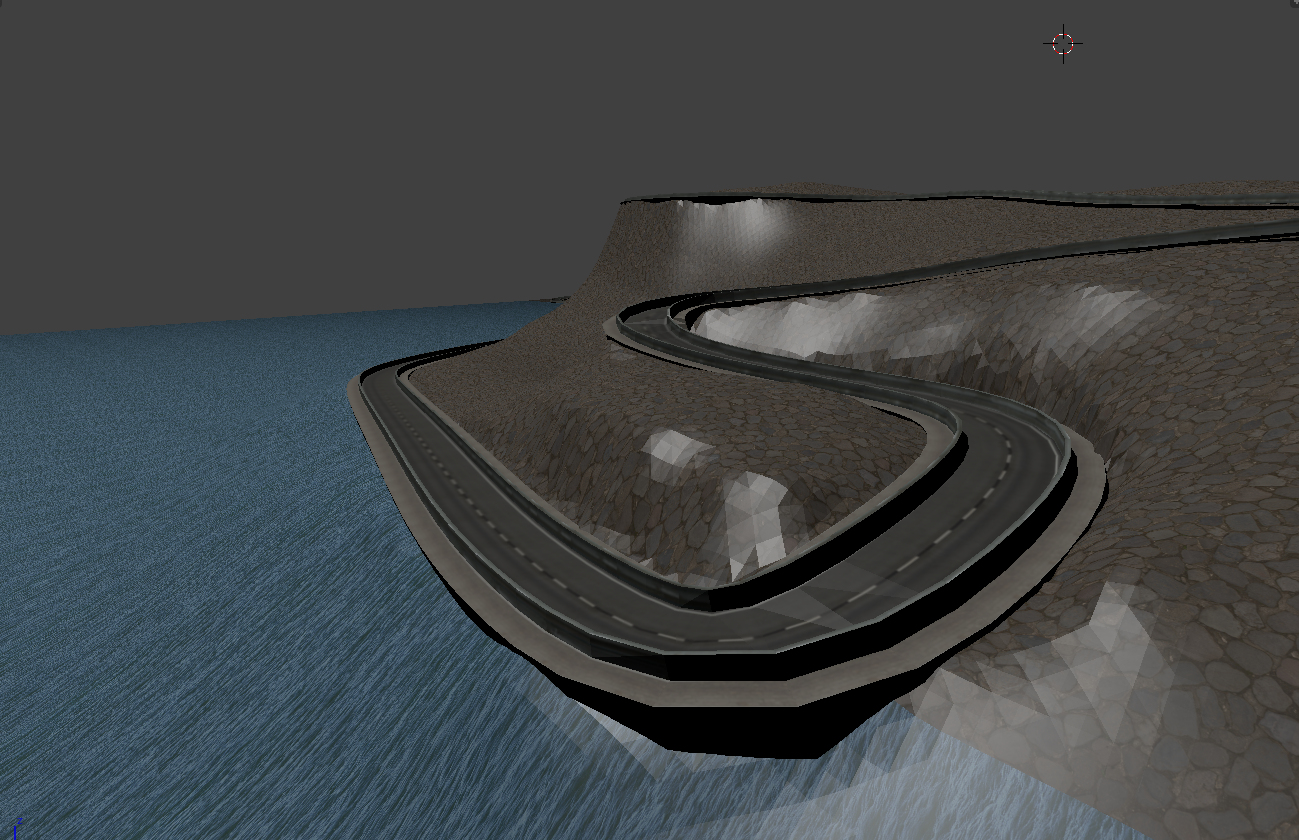
\includegraphics[width=0.495\textwidth]{MonacoElev04.png}}
	\caption{Diferentes vistas del circuito de F1 de Mónaco con elevaciones.} \label{fig:monacoelevvistas}
\end{figure}

Dado el carácter práctico de este escenario, y dado que ya existen prácticas desarrolladas con fines similares, procedemos a crear una variante del circuito, tanto el plano como el elevado, con una línea roja en el centro de su recorrido. Dicha línea servirá para realizar la práctica de control visual en la que es necesaria una referencia clara de un color determinado, siendo el rojo un color claramente diferente de cualquier componente del circuito como el asfalto o las vallas. Como podemos ver en la Figura \ref{fig:monacolinea} el circuito es idéntico en ambos casos salvo por la linea roja en el medio del asfalto. Para realizar esta modificación de la manera más eficiente y práctica realizamos unos pocos cambios al modelo original. Primero guardamos la escena con un nombre diferente para diferenciarlos. Después editamos la textura usada para crear el material del asfalto con un programa como GIMP\footnote{Siglas de “GNU Image Manipulation Program”, gratuito y de código abierto. \url{https://www.gimp.org/}} y le dibujamos esa línea roja. Después, en el nuevo fichero de Blender cambiamos, tanto en la textura como en el material asociado al asfalto, la imagen de fuente por la editada. Una vez hecho esto en ambos circuitos conseguimos esta variante más orientada a prácticas específicas. 

\begin{figure}[]
	\centering
	\subfigure[Mónaco plano.]{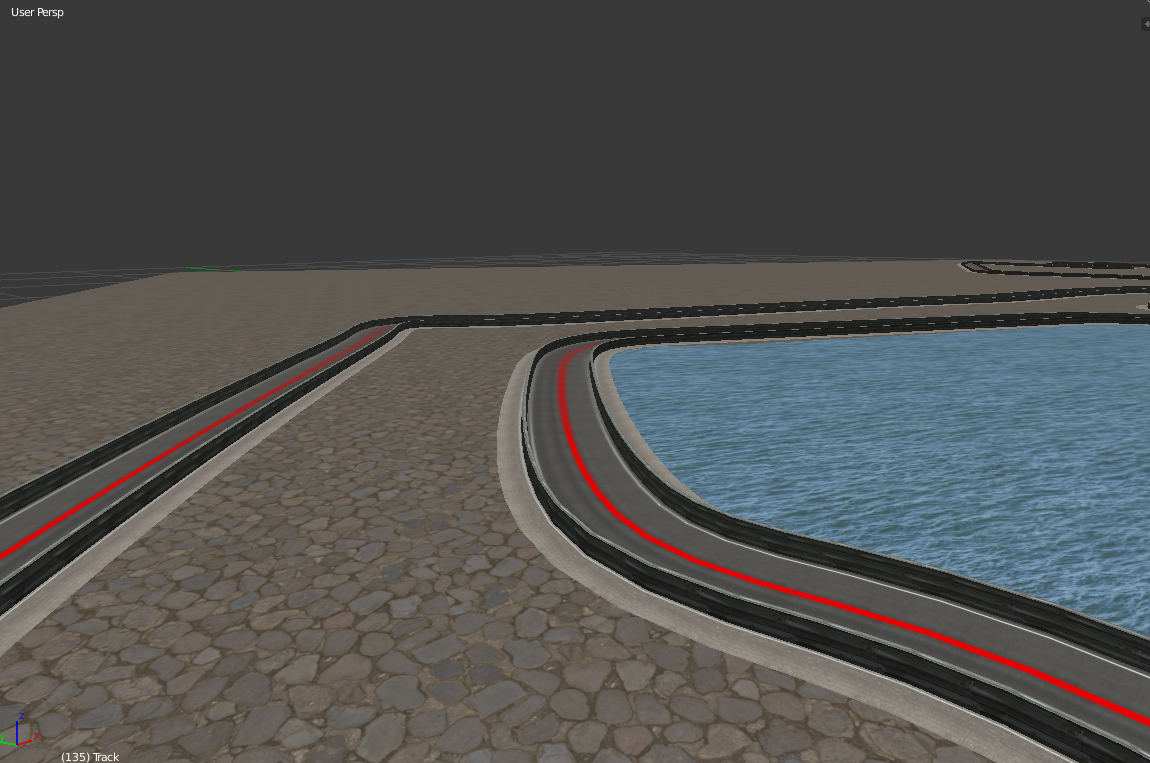
\includegraphics[width=0.49\textwidth]{monacolinea.png}}
	\subfigure[Mónaco con elevaciones.]{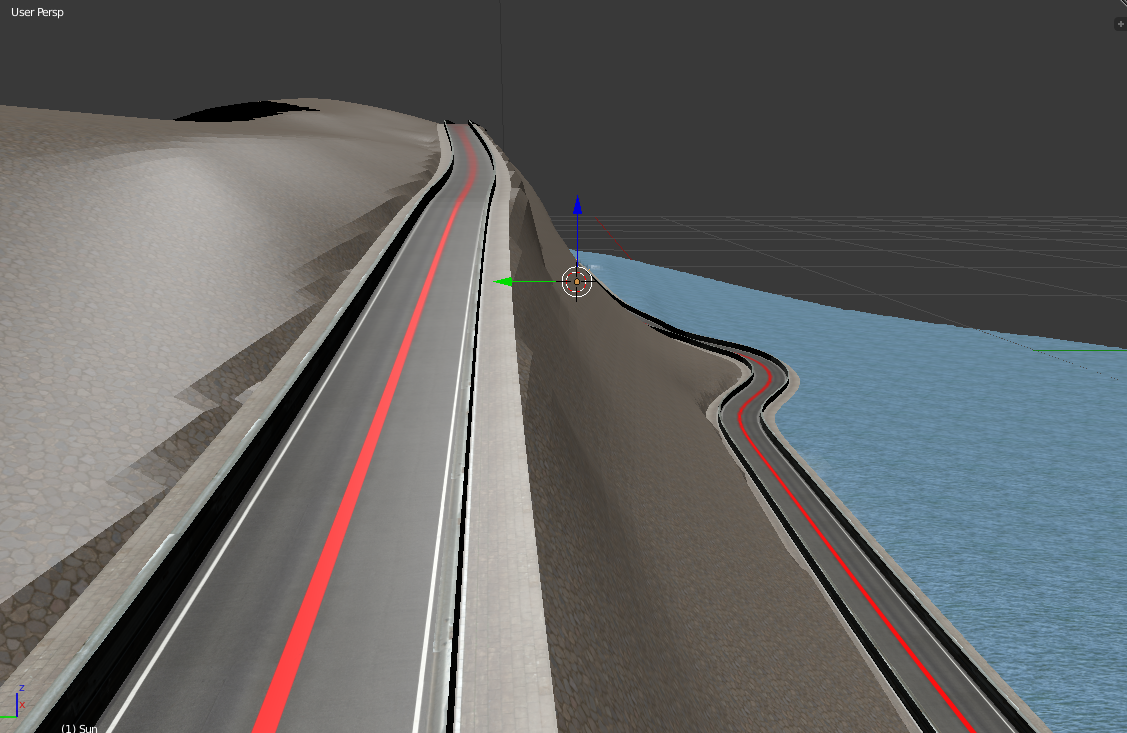
\includegraphics[width=0.5\textwidth]{monacoelevlinea.png}}
	\caption[Circuitos con una línea roja.]{Circuitos de mónaco editados para contener una línea roja en su trazado, tanto el plano (a) como el que contiene elevaciones (b).} \label{fig:monacolinea}
\end{figure}

\section{Mundos para Gazebo}
\label{sec:circarr_mundosparagazebo}

Ya hemos conseguido modelar dos escenarios, un circuito de Mónaco plano y otro con elevaciones, más realista. Pero aún no nos sirven, hemos de integrarlos en Gazebo para que puedan ser usados. Para ello estudiamos la estructura de los ficheros *.world de Gazebo, y vemos que se sirven de modelos en 3D en ficheros *.sdf y *.conf para componer los mundos. SDF\footnote{Página de SFD: \url{http://sdformat.org/}} es un formato XML que describe entornos y objetos para simuladores robóticos, visualización y control. Creado originalmente como parte de Gazebo, fué diseñado pensando en aplicaciones robóticas científicas, y ha evolucionado hasta convertirse en un formato robusto, estable y extensible capaz de describir objetos estáticos y dinámicos, terrenos, luces o físicas. 
Al analizar la estructura de los ficheros *.sdf observamos que importan los objetos que componen el mundo de otros ficheros en formatos como .mesh, .model, .dae, etc. Al comparar con otros mundo ya creados dentro de la plataforma JdeRobot vemos que muchos modelos están en formato .dae\footnote{Extensión asociada a los archivos Collada, esquema XML para transportar objetos 3D entre aplicaciones. \url{https://www.khronos.org/collada/}}. Así pues elegimos dicho formato para exportar el objeto desde Blender, comenzando primero con el circuito plano sin línea. Para ello hacemos click en el menú \textit{File}, \textit{Export}, \textit{Collada} (\textit{Figura \ref{fig:exportar}}).

\begin{figure}[h]
	\centering
	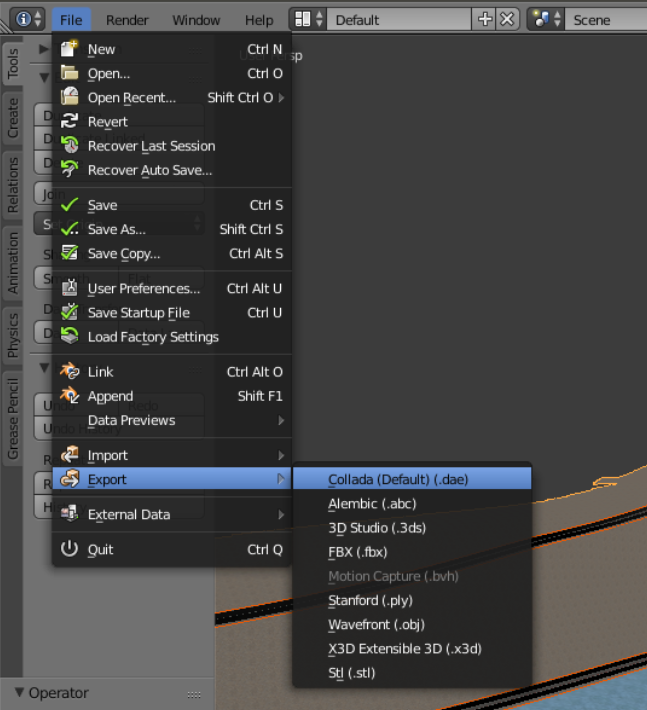
\includegraphics[width=0.6\textwidth]{exportar.png}
	\caption{Desplegable para exportar ficheros desde Blender.} \label{fig:exportar}
\end{figure}

En alguna versión de Blender esta opción no está disponible, por lo que hay que añadirla manualmente instalando desde fuente la extensión o buscar otra versión. En nuestro caso inicialmente instalamos la versión 2.76\textsubscript{b} y no tenía disponible esta opción. Optamos por instalar desde fuente la versión 2.78\textsubscript{c} que sí lo tiene. 

\begin{figure}[t]
	\centering
	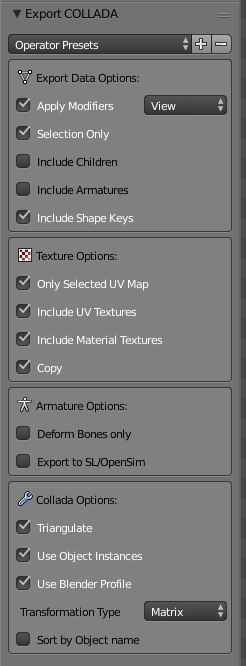
\includegraphics[width=0.3\textwidth]{exportcollada.png}
	\caption{Opciones de exportación de Collada.} \label{fig:exportcollada}
\end{figure}

Al seguir los pasos aparecemos en otra ventana de Blender donde nos pregunta la ruta donde exportar el archivo y el nombre del fichero, entre otros parámetros. Especialmente importantes son los que se aprecian en la Figura \ref{fig:exportcollada}. Si no se activan las casillas adecuadas se podrían producir errores en la exportación. Por ejemplo, dentro de \textit{Export Data Options} es necesario marcar tanto \textit{Apply Modifiers} como \textit{Selection Only}. La primera casilla sirve para no perder los modificadores aplicados a los objetos del escenario, como la curva o la rejilla aplicadas al segmento del circuito (\textit{Figura \ref{fig:monacosegmento}}). De no marcarlo podrían aparecer una fila de segmentos rectos y planos del circuito, o un circuito plano sobre las elevaciones, o un único segmento sin ninguno de los modificadores aplicados. 

El segundo es para exportar sólo los objetos seleccionados al hacer click en exportar. De esta manera podemos ayudarnos de múltiples objetos y mantenerlos en la escena para futuras modificaciones, o editar varios objetos a la vez en la misma escena pero exportarlos individualmente. De no marcar la casilla se exportarían todos los elementos de la escena. 

Dentro de \textit{Texture Options} se encuentran las opciones relaccionadas con las texturas. Aquí es necesario marcar las tres primeras casillas, \textit{Only Selected UV Map}, \textit{Include UV Textures}, \textit{Include Material Textures} y \textit{Copy}. Marcando la primera casilla se exportarán sólo las texturas de los objetos seleccionados, en lugar de todas las de la escena. La segunda y tercera casilla permiten exportar las texturas UV y los materiales usados respectivamente, de esta forma se mantienen las texturas que se veían en el modo de renderizado. Si simplemente asignamos una textura y no seguimos los pasos descritos anteriormente, en este paso Blender no las reconocería y no las exportaría junto con el resto del circuito, obteniendo así una figura sin imágenes en su superficie. 

La última casilla copia los archivos de las texturas a la carpeta de destino de la exportación, y los enlaza dentro del fichero .dae. De esta forma se pueden copiar los archivos resultantes a cualquier otro dispositivo sin perder ningún dato por el camino o hacer más configuración manual. Las secciones de \textit{Armature Options} y \textit{Collada Options} no son relevantes en nuestro caso, y con dejar las casillas marcadas por defecto es suficiente.

Una vez tenemos exportado el circuito a un fichero .dae, creamos el fichero .sdf que importaremos en el mundo de Gazebo. El fichero finalizado tendrá el siguiente contenido:

\lstset{language=xml}
\begin{lstlisting}
<?xml version='1.0'?>
<sdf version="1.4">
<model name="monaco">
	<static>true</static>
	<link name="monaco">
		<pose>0 0 0 0 0 0</pose>
		<collision name="collision">
			<geometry>
				<mesh>
					<scale>15 15 15</scale>
					<uri>model://monaco/meshes/CircuitoMonaco.dae</uri>
				</mesh>
			</geometry>
		</collision>
		<visual name="visual">
			<geometry>
				<mesh>
					<scale>15 15 15</scale>
					<uri>model://monaco/meshes/CircuitoMonaco.dae</uri>
				</mesh>
			</geometry>
		</visual>
	</link>
</model>
</sdf>
\end{lstlisting}

Dentro de este fichero podemos diferenciar claramente el campo \textit{link} entre las líneas 5 y 23. En este campo se importan los archivos y configuraciones que componen el modelo sdf. Podemos ver tres campos: \textit{pose}, \textit{collision} y \textit{visual}. El primero define la posición y la orientación del objeto. En nuestro caso, como estamos creando el modelo del mundo donde se situarán los demás objetos, podemos dejar cualquiera con tal de que esté minimamente centrado en el mundo. El segundo define las barreras de colisión con los demás objetos del mundo. Es importante dado que, de no incluirlo, Gazebo trataría el objeto como si de un holograma se tratase, permitiendo que cualquier otro objeto lo atravesase sin problemas. Y el tercero define la parte que se ve del objeto. Si no lo definimos obtendremos un circuito invisible. Ambos campos tienen definidos unos valores de \textit{scale}. Esto es así para mantener una cohesión con los demás mundos creados en JdeRobot y con los vehículos existentes. Es importante también el campo de la línea 4, \textit{static}, con valor \textit{true}. Este campo fuerza al circuito a quedarse inmóvil en el espacio de Gazebo y actuar como suelo para los coches. De no definirlo o no asignarle el valor \textit{true}, obtendremos un circuito que al comenzar la simulación de Gazebo caerá al vacío, junto con los demás objetos.

Para cumplir con el estándar de SDF es necesario también crear un fichero de configuración como este:
\lstset{language=xml}
\begin{lstlisting}
<?xml version="1.0"?>
	<model>
	<name>Monaco flat</name>
	<version>1.0</version>
	<sdf version='1.5'>model.sdf</sdf>

	<author>
		<name>Alvaro Villamil</name>
	</author>

	<description>
		The F1 Monaco track without elevations.
	</description>
</model>
\end{lstlisting}

De este fichero, de extensión .config, SDF extrae información como el nombre del modelo, la versión usada para crearlo, la descripción del mismo, el archivo al cual aplicar esta configuración o el autor.

A continuación estructuramos los ficheros para que mantengan coherencia con el resto de modelos de JdeRobot. De tal forma creamos una carpeta con el nombre del modelo, en este caso \textit{monaco}, y dentro de ella situamos los archivos \textit{model.config} y \textit{model.sdf} y una carpeta que llamamos \textit{meshes}. Dentro de esta carpeta guardamos el archivo \textit{CircuitoMonaco.dae} y todas las texturas que necesita nuestro modelo, tal y como las exportó Blender.

El siguiente paso es crear el fichero \textit{monaco.world}, el cual pasaremos como argumento a Gazebo al lanzarlo para que cargue nuestro mundo. Para decirle a Gazebo que queremos cargar nuestro circuito creamos el campo \textit{include} de las líneas 7 a 10. De esta manera le decimos que cargue el modelo \textit{monaco} y lo coloque en una posición en el mundo. También creamos un sol estándar de Gazebo en otro campo \textit{include}. Al probar a lanzar Gazebo con esta configuración vemos que la escena queda muy oscura y decidimos añadir dos \textit{light}, dos luces direccionales que además aportarán sombras y dinamismo al mundo. Para no crear una carga excesiva de trabajo de simulación hacemos que ambas luces sean idénticas, potenciando el efecto sin crear varias sombras ni reflejos innecesarios. El contenido final de dicho fichero es éste:
\\
\\
\\
\lstset{language=xml}
\begin{lstlisting}
<?xml version="1.0"?>
<sdf version="1.4">
	<world name="default">
		<include>
			<uri>model://sun</uri>
		</include>
		<include>
			<uri>model://monaco</uri>
			<pose>0 0 0 0 0 0</pose>
		</include>

		<light name='user_directional_light_0' type='directional'>
			<pose frame=''>0.467439 -3.3788 2.45574 0.487341 -0 0</pose>
			<diffuse>0.5 0.5 0.5 1</diffuse>
			<specular>0.1 0.1 0.1 1</specular>
			<direction>0.1 0.1 -0.9</direction>
			<attenuation>
				<range>20</range>
				<constant>0.5</constant>
				<linear>0.01</linear>
				<quadratic>0.001</quadratic>
			</attenuation>
			<cast_shadows>1</cast_shadows>
		</light>
		<light name='user_directional_light_1' type='directional'>
			<pose frame=''>0.467439 -3.3788 2.45574 0.487341 -0 0</pose>
			<diffuse>0.5 0.5 0.5 1</diffuse>
			<specular>0.1 0.1 0.1 1</specular>
			<direction>0.1 0.1 -0.9</direction>
			<attenuation>
				<range>20</range>
				<constant>0.5</constant>
				<linear>0.01</linear>
				<quadratic>0.001</quadratic>
			</attenuation>
			<cast_shadows>1</cast_shadows>
		</light>

	</world>
</sdf>
\end{lstlisting}

Para incorporarlo al conjunto de mundos y modelos de JdeRobot, primero comprobamos en nuestro ordenador que funciona correctamente. Para ello copiamos la carpeta \textit{monaco} con los archivos correspondientes al modelo dentro de la carpeta \textit{JdeRobot/src/drivers/gazeboserver/models}, y el fichero \textit{monaco.world} dentro de la carpeta \textit{JdeRobot/src/drivers/gazeboserver/worlds}. Al lanzar Gazebo con nuestro mundo como argumento no da ningún error y aparece el circuito correctamente. Una vez probado que todo funciona repetimos el proceso para cada circuito, obteniendo cuatro modelos y cuatro mundos, los correspondientes al circuito plano, al circuito con elevaciones, al circuito plano con la línea roja y al circuito con elevaciones con la línea roja. 

Sin embargo, las precauciones tomadas no han sido suficientes y los circuitos de Mónaco con elevaciones llevan una gran carga gráfica que hace que la simulación se mueva lenta. Para disminuir esta carga recortamos parte de la rejilla que sirve de fondo, reduciendo la zona del mar y la zona alta detrás del circuito. Son zonas lejanas al trazado que no van a disminuir la apariencia general, pero si a mejorar el rendimiento computacional. Una vez hecho este cambio comprobamos que la simulación en Gazebo se mueve con soltura y nos permite añadir objetos sin afectar al rendimiento. 

\begin{figure}[h]
	\centering
	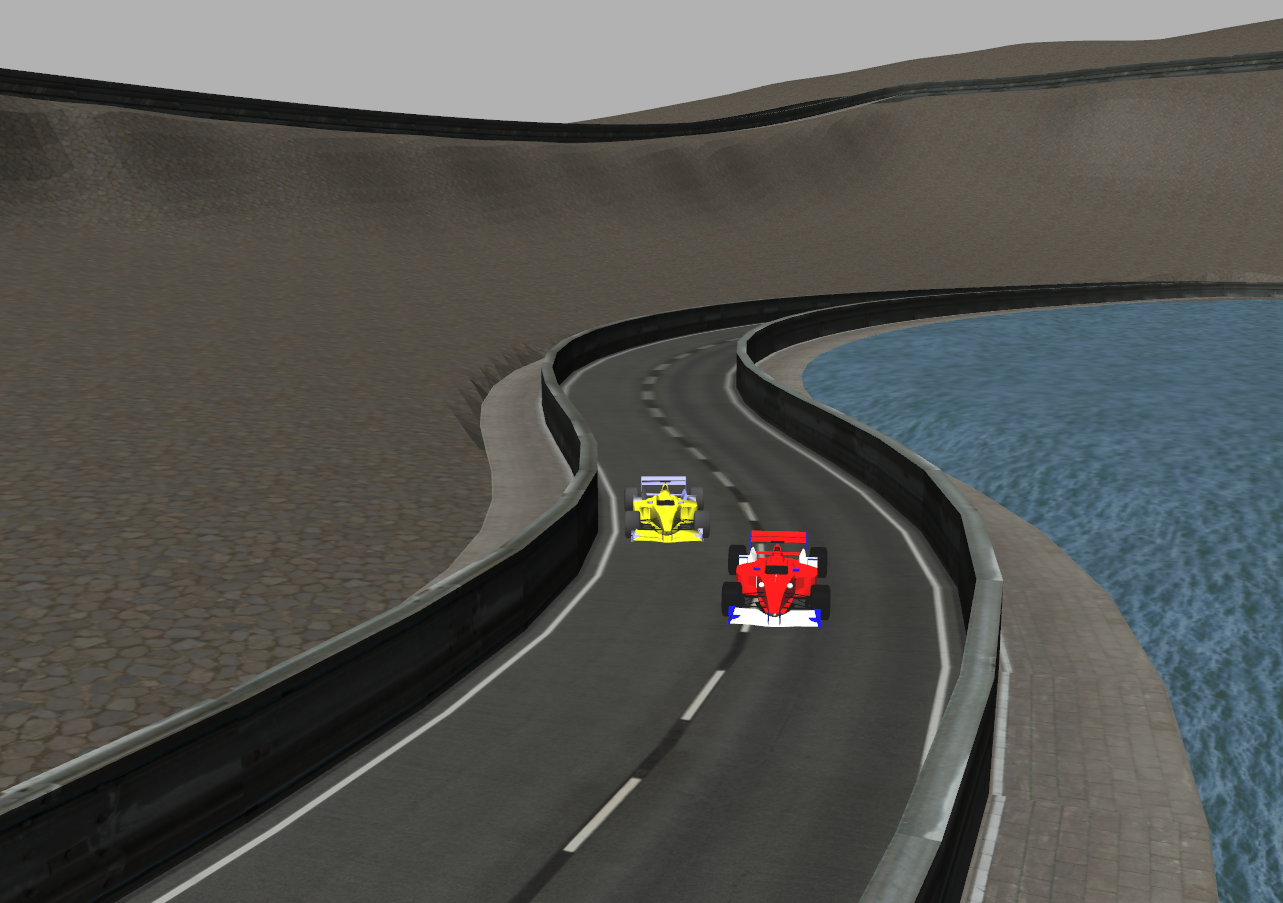
\includegraphics[width=0.75\textwidth]{MonacoElev08.png}
	\caption{Coches recorriendo el circuito de Mónaco.} \label{fig:monacocoches}
\end{figure}

Cuando ya hemos comprobado que con ninguno de los cuatro mundos se producen errores procedemos a hacer un \textit{pull} al repositorio oficial de JdeRobot\footnote{\url{https://github.com/JdeRobot/JdeRobot}} en GihHub. De esta forma logramos incorporar nuestros progresos al código oficial de JdeRobot, y que cualquiera que se descargue esta plataforma pueda disfrutar de los mundos que hemos creado. En la figura \ref{fig:monacocoches} podemos observar el resultado en Gazebo con coches circulando por el circuito como si de una práctica académica se tratase. También comprobamos que la fluidez del mundo al aumentar la carga de trabajo sigue siendo satisfactoria, y va a permitir realizar diferentes tipos de prácticas.


\chapter{Brazo robótico}
\label{ch:BrazoRobotico}

En este capítulo vamos a estudiar el comportamiento y la estructura de un brazo robótico para luego crear un controlador de bajo nivel. Dado que el objetivo no es crear un brazo, sino trabajar sobre uno ya diseñado, comenzamos buscando uno sobre el cual realizar el estudio. Debido a un cambio en la distribución de los paquetes de ROS entre las versiones Indigo y Jade, la mayoría de brazos manipuladores encontrados son antiguos y dan muchos problemas de instalación y configuración en las versiones más modernas. A partir de Indigo, los paquetes que forman ROS Industrial se han separado del núcleo de ROS no están mantenidos por ROS, por lo que el desarrollo y la corrección de errores es más lenta. Puesto que queremos realizar el trabajo sobre ROS Kinetic y Gazebo 7 necesitamos encontrar un brazo que funcione bajo estas versiones. Tanteamos el uso de varios modelos:
\begin{itemize}
	\item PR2: De la empresa Clear Path Robotics\footnote{\url{https://www.clearpathrobotics.com/}}, responsables también del kobuki o turtlebot. Se trata de un robot con apariencia de androide (\textit{Figura \ref{fig:pr2}}). Se compone de una base con ruedas, dos brazos y una cabeza con diferentes sensores visuales, siendo los brazos donde centraríamos nuestra atención. Cuando miramos su página de ROS\footnote{\url{http://wiki.ros.org/Robots/PR2}} observamos que no da soporte más allá de Indigo, lo cual puede suponer un problema.
	\begin{figure}[h]
		\centering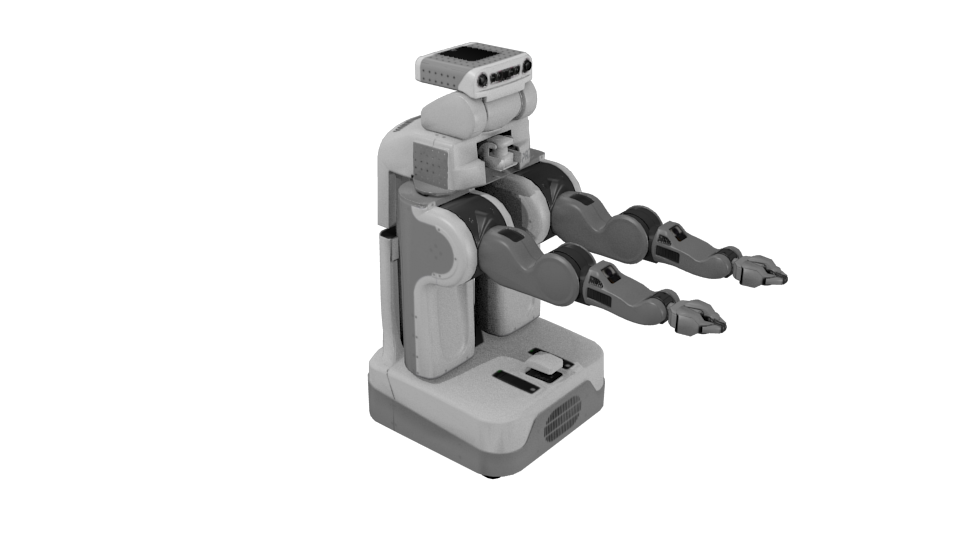
\includegraphics[width=0.5\textwidth]{pr2.png}
		\caption{Robot PR2.}
		\label{fig:pr2}
	\end{figure}
	\item kuka: La empresa Kuka\footnote{\url{https://www.kuka.com/}} fabrica diversos brazos mecánicos y robots industriales. Hay varios modelos disponibles para su uso con Gazebo y ROS, y todos tienen en común el brazo que monta el robot de la Figura \ref{fig:kuka}, aunque la plataforma donde se apoya el brazo puede ser diferente o no estar. En su página de ROS\footnote{\url{http://wiki.ros.org/kuka}} vemos que soporta las versiones de Indigo y Kinetic, pero mediante la instalación del paquete externo ROS-Industrial\footnote{\url{http://wiki.ros.org/Industrial}}.
	\begin{figure}[h]
		\centering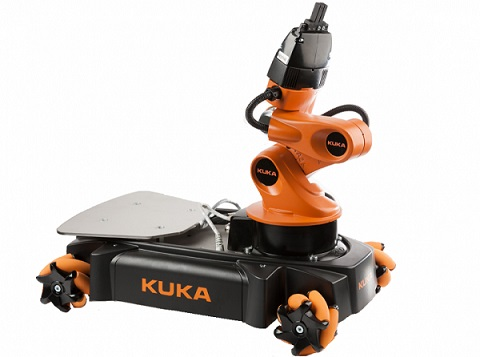
\includegraphics[width=0.4\textwidth]{kuka.jpg}
		\caption{Robot kuka.}
		\label{fig:kuka}
	\end{figure}
	\item ur10: De la empresa Universal Robots\footnote{\url{https://www.universal-robots.com/es/}}. Es un brazo simple (\textit{Figura \ref{fig:ur10}}), al igual que sus hermanos el ur3 y el ur5. La diferencia entre estos no va más allá del tamaño y fuerza del robot. En su página de ROS\footnote{\url{http://wiki.ros.org/ur_gazebo}} observamos que no da soporte más allá de Indigo, lo cual puede suponer un problema.
	\begin{figure}[h]
		\centering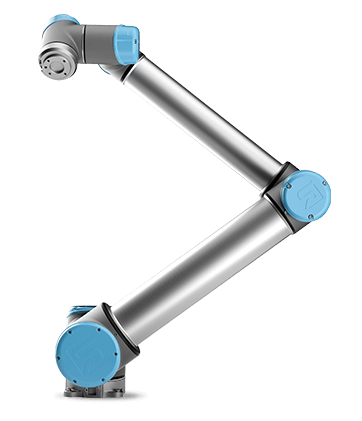
\includegraphics[width=0.3\textwidth]{ur10.png}
		\caption{Robot ur10.}
		\label{fig:ur10}
	\end{figure}
\end{itemize}

Probamos los brazos bajo la última versión de Gazebo y de ROS recurriendo a la extensa comunidad de ROS en busca de soluciones para incorporar los brazos a la última versión. Algunas de las soluciones propuestas y probadas por nosotros son la instalación manual desde fuente, la compilación manual del código fuente, paquetes alternativos de usuarios que han resuelto los problemas de compatibilidad o interfaces de usuarios para que el robot se comunique con las librerías actuales. Después de probar muchas de estas soluciones, y de intentar solucionar los problemas por nuestra cuenta, vemos que ninguno de ellos llega a funionar de forma correcta bajo nuestros requisitos.

Recurrimos a los escenarios de ARIAC (\textit{Sección \ref{sec:inf_ariac}}) para desarrollar nuestro trabajo. Como podemos ver en la Figura \ref{fig:ariac01} se trata de un escenario industrial, con un brazo ur10 situado sobre un carril que le permite desplazarse. Nos centramos en esta parte del escenario y del código, estudiando cómo está construido y cómo funciona. Es de gran ayuda la página de documentación de ARIAC\cite{ariacwiki} donde se detallan las interfaces de comunicación de los elementos del escenario.

Para poder avanzar y comenzar a probar cosas sobre el funcionamiento del brazo, necesitamos comprender mejor cómo funciona ROS. 

\section{Hablando ROS}
\label{sec:br_hablandoros}

Para aprender el funcionamiento de ROS vamos a la documentación oficial\cite{roswiki}. Una vez allí nos damos cuenta de que básicos que conocer para entender ROS son los \textit{topics}, los \textit{nodes} y  los \textit{messages}. 

Los \textit{nodes} son los procesos ejecutables, en nuestro caso escritos en Python, que se combinan entre sí siguiendo un esquema de grafos. Se comunican unos con otros mediante \textit{topics}, servicios y acciones. Está pensado para que cada tarea dentro del robot la ejecute un nodo, facilitando APIs y canales de comunicación que hacen que el conjunto de código sea mucho mas sencillo de depurar y de utilizar. ROS facilita comandos de terminal como \textit{rosnode list}, que muestra una lista de los nodos activos. Estos comandos son de gran ayuda para entender el funcionamiento del brazo.

Los \textit{topics} son \textit{buses}diferenciables mediante los cuales los nodos intercambian \textit{ROS messages} o mensajes. Normalmente los \textit{topics} y los nodos no se preocupan del destinatario de los mensajes. Los nodos se subscriben a los topics, y pueden publicar información en el topic haciendo \textit{publish}, por ejemplo un sensor de temperatura o de proximidad, o recibir información del topic haciendo \textit{subscribe}, para tomar decisiones o procesar los datos recibidos. Son canales de comunicación unidireccionales. Utilizan \textquotedblleft tipado fuerte\textquotedblright  mediante el tipo de \textit{ROS message} que transmiten, de forma que un tipo de mensaje erróneo no se puede transmitir por el \textit{topic} y no producirá fallos en otros nodos. ROS facilita comandos de terminal como \textit{rostopic list} y \textit{rostopic echo /topic\_name}. El primero muestra una lista con los \textit{topics} activos, y el segundo permite ver el flujo de mensajes a través del topic deseado. Ambos son una ayuda inestimable para conseguir entender, y más tarde replicar, la comunicación con el brazo.

\begin{figure}[]
	\centering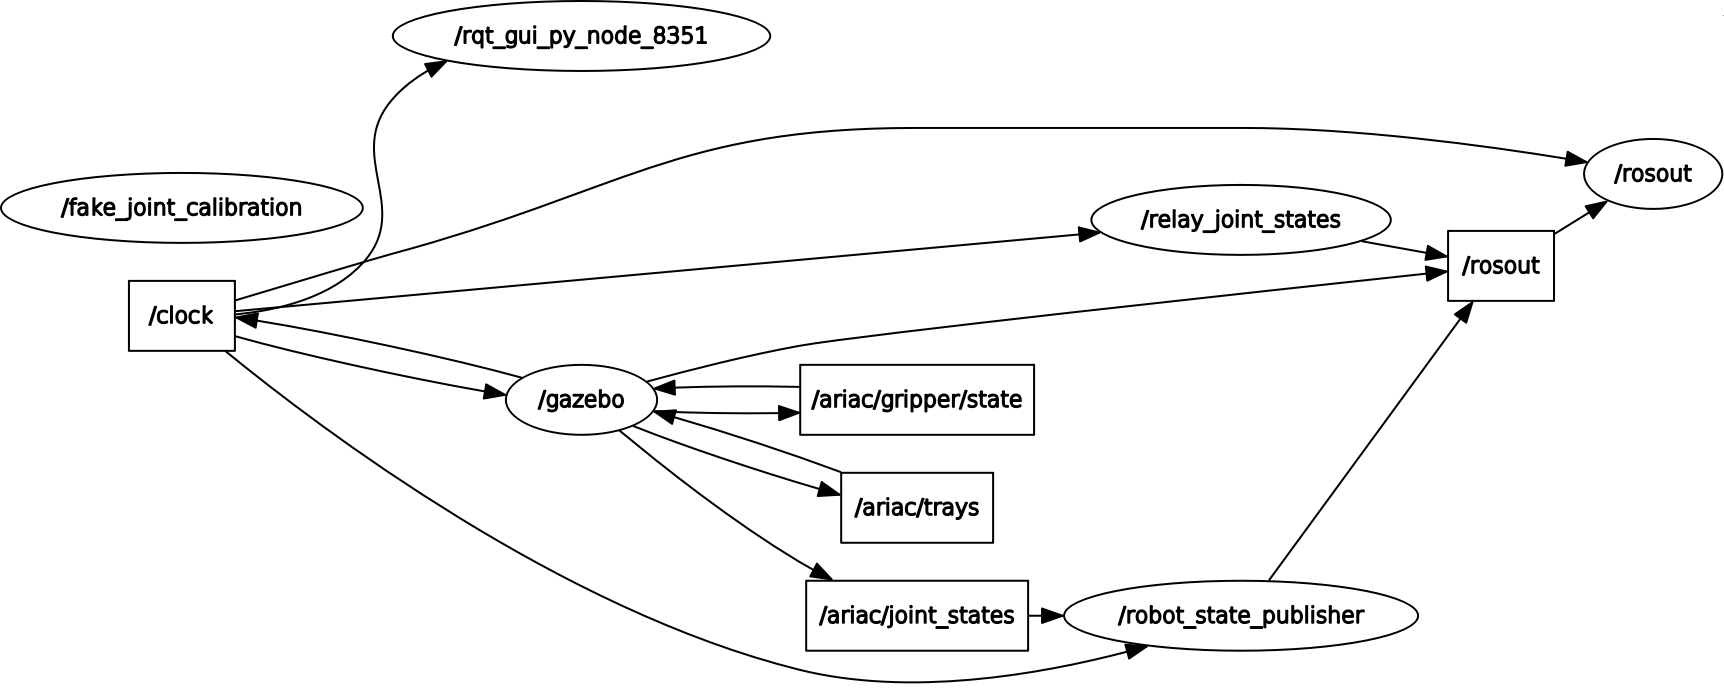
\includegraphics[width=1\textwidth]{Brazo10a.png}
	\caption{Grafo de los \textit{nodes} y \textit{topics} de ARIAC.}
	\label{fig:ariacgraph1}
\end{figure}

Los servicios son canales bidireccionales de comunicación entre nodos. Esto quiere decir que cuando se envía un mensaje, el nodo destino debe enviar otro de respuesta, o la comunicación no tiene éxito. Las acciones son un método de comunicación mas directo, como si de una llamada a procedimiento se tratase. Ninguno de estos medios son usados para enviar órdenes al brazo, por lo que no profundizamos en ellos.

Los \textit{ROS messages} contienen la información que los nodos se envían mediante los \textit{topics}. Se trata de estructuras de datos con campos fijos, que soportan tanto tipos de datos primitivos (enteros, \textit{floats}, \textit{boleanos}, etc) como arrays de estos tipos de datos. Estas estructuras están predefinidas en la mayoría de casos comunes, pero se pueden definir nuevas usando archivos en formato .msg donde se específique la estructura de datos del mensaje

Una vez conocemos los elementos de comunicación probamos cómo se produce, creando un nodo \textit{publisher} y otro \textit{subscriber} y haciendo que hablen entre sí. Mediante los diferentes comandos de terminal que proporciona ROS comprobamos el correcto funcionamiento de los mismos. 

Una vez entendemos el funcionamiento de ROS lanzamos el mundo de ARIAC. A través de los comandos visualizamos la lista de nodos y topics disponibles. Nos servimos de una herramienta de ROS para obtener un grafo con la relación entre todos ellos y tener una idea clara del funcionamiento y la relación entre los elementos del brazo. Para ellos ejecutamos en la terminal \textit{rosrun rqt\_graph rqt\_graph} y obtenemos la Figura \ref{fig:ariacgraph1}. En dicha figura, los elementos redondos son nodos y los cuadrados son \textit{topics}, y las flechas establecen la relación entre ellos. Si la flecha apunta hacia un \textit{node} desde un \textit{topic} quiere decir que el nodo es ta subscrito a ese \textit{topic}. Si por el contrario la flecha va desde un \textit{node} a un \textit{topic} quiere decir que el nodo publica en ese \textit{topic}.

Aunque ya nos da una idea muy clara de la organización de los nodos y topics, la herramienta \textit{rqt\_graph} nos permite agruparlos por nombres. Dado que hay varios \textit{topics} cuyo nombre es \textquotedblleft /ariac/nombre\textquotedblright , \textit{rqt} incluye a todos los que tienen ese formato en el nombre en la caja ARIAC. De esta forma la caja ariac hace referencia a todos los nodos y \textit{topics} que comparten el nombre ariac.

\begin{figure}[h]
	\centering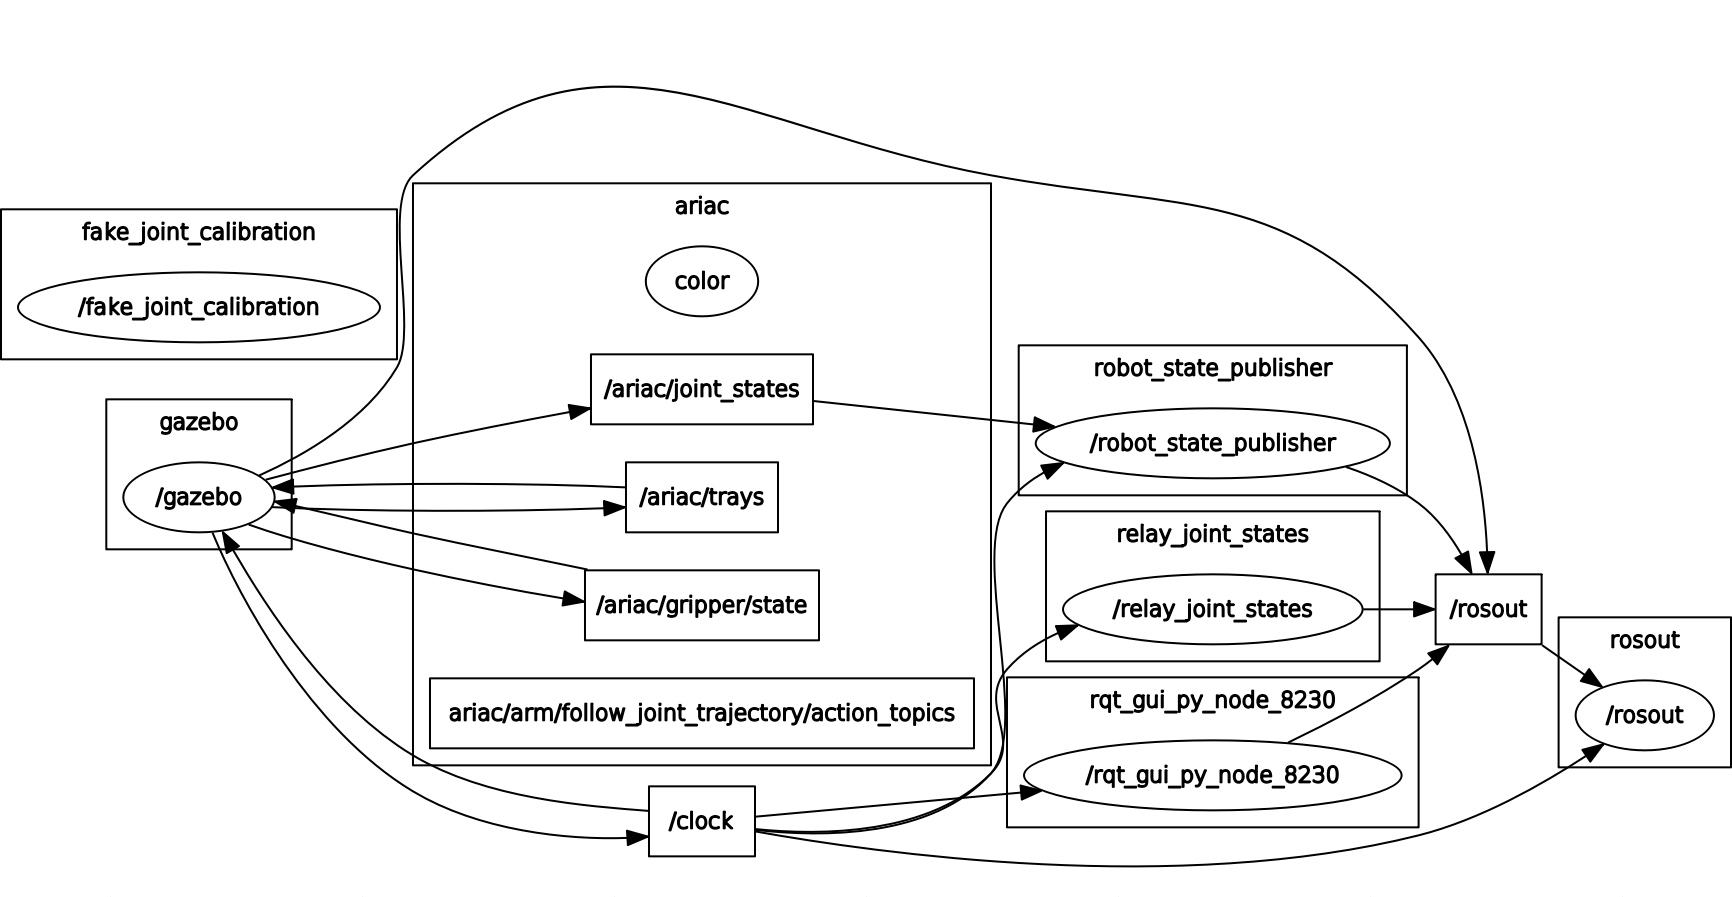
\includegraphics[width=1\textwidth]{Brazo10.png}
	\caption{Grafo de los \textit{nodes} y \textit{topics} de ARIAC.}
	\label{fig:ariacgraph2}
\end{figure}

En esa figura podemos diferenciar varios bloques importantes. En el centro del grafo se sitúan los \textit{topics} y nodos referentes al mundo ariac, A su izquierda se encuentra el nodo principal de Gazebo. Encima de éste y a la derecha del bloque ariac hay varios grupos que sirven de apoyo para el entorno ariac: \textit{fake\_joint\_calibration}, \textit{robot\_state\_publisher} y \textit{relay\_joint\_states}.
Debajo de ariac se encuentra el topic \textquotedblleft /clock\textquotedblright  , que sirve de referencia para todos los elementos de la simulación. A la derecha de este está el nodo de \textit{rqt} que nos permite obtener esta imagen. A la derecha del grafo hay diversos nodos y topics de \textit{rosout}. Se trata de la consola de \textit{log} de ROS, donde se anotan los sucesos o errores de los diferentes procesos ejecutados.

\section{Controlando el Brazo}
\label{sec:br_controlandobrazo}

Una vez tenemos este esquema en la cabeza acudimos tanto al código de ARIAC como a su documentación para ver qué hace cada nodo y cada topic, qué partes controlan el brazo y cómo podemos comunicarnos con ellas. De esta forma descubrimos dos \textit{topics} calve para poder controlar el brazo:
\begin{itemize}
	\item /ariac/joint\_states: En este \textit{topic} se publica la información relativa las posiciones de las articulaciones del brazo. Por este \textit{topic} se envían mensajes de tipo \textit{sensor\_msgs/JointState Message}, que veremos más adelante. Nos subscribiremos a este \textit{topic} para conocer la posición inicial del brazo y de sus articulaciones.
	
	\item /ariac/arm/command: Por este \textit{topic} se envía al brazo la posición a la que quieres moverlo mediante mensajes del tipo \textit{trajectory\_msgs/JointTrajectory Message}, que veremos más adelante. necesitamos publicar en este \textit{topic} para enviar órdenes al brazo.
	
\end{itemize}

Los demás \textit{topics} tienen otras funciones que no necesitamos para conseguir nuestro objetivo.

Los mensajes descritos anteriormente tienen la siguiente estructura:
\begin{itemize}
	\item \textit{sensor\_msgs/JointState Message}:
	\begin{lstlisting}
	std_msgs/Header header
	string[] name
	float64[] position
	float64[] velocity
	float64[] effort
	\end{lstlisting}
	\item \textit{trajectory\_msgs/JointTrajectory Message}:
	\begin{lstlisting}
	std_msgs/Header header
	string[] joint_names
	trajectory_msgs/JointTrajectoryPoint[] points
	\end{lstlisting}
\end{itemize}

Ambos mensajes comienzan con un \textit{Header} de tipo \textit{std\_msg/Header}. Este es un tipo de mensaje estándar de ROS, que necesitan todos los mensajes para que pueda establecerse la comunicación, y se crea automáticamente al enviar el mensaje. No necesitamos crearlo para poder enviar mensajes y no necesitamos extraerlo al recibirlos, por lo que no nos preocupamos por el.

El primer tipo de mensaje lo componen varios \textit{arrays} de datos primitivos. El primero de ellos es un \textit{array} de \textit{strings}. Los \textit{strings} son cadenas de caracteres, como palabras o frases. Este campo lo componen los nombres de las articulaciones del brazo, que son:
\begin{itemize}
	\item elbow\_joint : Esta es la articulación del codo, la del medio del brazo.
	
	\item linear\_arm\_actuator\_joint : Esta no es una articulación propiamente dicha, sino que se refiere a la posición del brazo en el carril sobre el que está situado.
	
	\item shoulder\_lift\_joint : Esta es la articulación del hombro, es decir, la más cercana a su base. En concreto esta es la articulación que controla la elevación del brazo. Realiza giros sobre un imaginario eje y.
	
	\item shoulder\_pan\_joint : Esta es la articulación del hombro, es decir, la más cercana a su base. En concreto esta es la articulación que controla la orientación del brazo y nos permite girarlo. Realiza giros sobre un imaginario eje z.
	
	\item wrist\_1\_joint : Esta es la articulación de la muñeca, la más alejada de la base. En concreto esta articulación controla la elevación de la muñeca y nos permite subirla y bajarla. Realiza giros sobre un imaginario eje y.
	
	\item wrist\_2\_joint : Esta es la articulación de la muñeca, la más alejada de la base. En concreto esta articulación controla el giro de la muñeca y nos permite rotarla verticalmente. Realiza giros sobre un imaginario eje z.
	
	\item wrist\_3\_joint : Esta es la articulación de la muñeca, la más alejada de la base. En concreto esta articulación controla el giro de la mano y nos permite rotar la muñeca horizontalmente. Realiza giros sobre un imaginario eje x.
	
	\item vacuum\_gripper\_joint : Esta articulación hace referencia a una pinza de vacío que se puede acoplar a la articulación de la muñeca del brazo, pero en nuestro caso no la incorpora y no necesitamos asignarle valores
\end{itemize}

En la Figura \ref{fig:brazoarticulaciones} podemos situar visualmente las articulaciones en el brazo, con la diferencia de que la articulación \textit{Base Joint} de la imágen en ARIAC se llama \textit{shoulder\_pan\_joint}. Todas articulaciones tienen definida su posición en radianes y unos límites de giro entre 6,28 y -6,28 en su mayoría. Esto quiere decir que cada articulación del brazo puede realizar dos giros completos si fuese necesario, pero los choques con los elementos de escenario limitan los movimientos.

\begin{figure}[]
	\centering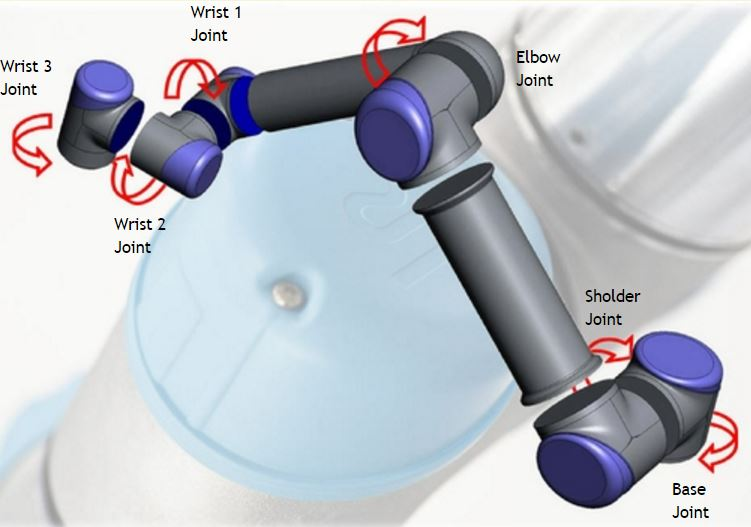
\includegraphics[width=0.6\textwidth]{brazoarticulaciones.jpg}
	\caption{Detalle de las articulaciones del brazo.}
	\label{fig:brazoarticulaciones}
\end{figure}

Los siguientes campos del mensaje son \textit{arrays} de \textit{floats} (números) de posiciones, velocidades y esfuerzos. Dan información de la posición de cada articulación, la velocidad a la que se mueven, y el esfuerzo o fuerza que poseen en el momento de envío del mensaje, por lo que son arrays de ocho posiciones y en cada una está la información relativa a la articulación en la posición homóloga en el array de nombres. A nosotros nos interesa el primer \textit{array} para conocer la posición inicial de las articulaciones.

Para ver mejor la estructura del mensaje lanzamos el mundo de ARIAC y ejecutamos el comando de terminal \textit{rostopic echo /ariac/joint\_states}, obteniendo en texto en la terminal la estructura de datos de este mensaje:

\begin{lstlisting}
---
header: 
seq: 265
stamp: 
secs: 5
nsecs: 322000000
frame_id: ''
name: ['elbow_joint', 'linear_arm_actuator_joint', 'shoulder_lift_joint', 'shoulder_pan_joint', 'wrist_1_joint', 'wrist_2_joint', 'wrist_3_joint', 'vacuum_gripper_joint']
position: [1.5072954794978815, 0.04169673392358113, -0.3793140712872205, 3.217984505432054, 3.085834205511564, -1.6130778569148077, -0.00793595855568796, 0.0]
velocity: [0.027474972846918494, 0.007286219434794008, 0.05461882849916373, 0.0316967471028743, 0.1957558318356749, -1.091011699832568, -8.054309845386587, 0.0]
effort: [150.0, -184.23945050318943, 330.0, 167.6704306272329, 0.0, 5.601291580407757, -5.541011517572109, 0.0]
---
\end{lstlisting}

El \textit{header} o cabecera ocupa las primeras siete líneas, y refleja datos como el tiempo de simulación o el número de mensaje, ninguno de ellos relevante para nosotros. A continuación nos encontramos los cuatro \textit{arrays}: \textit{name} para los nombres de las articulaciones, \textit{position} para las posiciones, \textit{velocity} para las velocidades y \textit{effort} para las fuerzas. Este mensaje es el que recibiremos y que deberemos procesar para obtener la posición inicial del brazo.

El segundo tipo de mensaje lo componen un \textit{array} de \textit{strings} y otro campo llamado \textit{points} compuesto por otro tipo de mensaje, el tipo \textit{trajectory\_msgs/JointTrajectoryPoint}. El primer \textit{array} hace referencia a los nomvres de las articulaciones, pero en este mensaje se llama \textit{joint\_names} Como podemos ver a continuación, este tipo de mensaje está formado por \textit{arrays} de números de forma muy similar a los del primer mensaje:
\begin{lstlisting}
float64[] positions
float64[] velocities
float64[] accelerations
float64[] effort
duration time_from_start
\end{lstlisting}
Tenemos un \textit{array} para las posiciones, otro para las velocidades, otro para las aceleraciones, otro para las fuerzas, y un último campo de tipo \textit{duration} para especificar el número de segundos desde el inicio para ejecutar los movimientos. Nosotros usaremos tanto el \textit{array} de nombres com el de posiciones, así como el campo para establecer el tiempo inicial de la orden. Los demás campos no son necesarios para el correcto funcionamiento del brazo.

De la misma forma que con el mensaje anterios, arrancamos la simulación y ejecutamos en la terminal el comando \textit{rostopic echo /ariac/arm/commander} para obtener en texto el contenido de los mensajes que pasan por este topic. Nos servimos de los tutoriales para dar órdenes sencillas a través de comandos de terminal y poder capturar el contenido de estos mensajes:
\begin{lstlisting}
---
header: 
seq: 59
stamp: 
secs: 0
nsecs:         0
frame_id: ''
joint_names: ['elbow_joint', 'linear_arm_actuator_joint', 'shoulder_lift_joint', 'shoulder_pan_joint', 'wrist_1_joint', 'wrist_2_joint', 'wrist_3_joint']
points: 
- 
positions: [1.510634135925831, 1.4199980429372933e-06, -1.1286545928274752, 3.140002031709801, 3.772089274964015, -1.5100101552695162, 4.0770707014914365e-06, 0.0]
velocities: []
accelerations: []
effort: []
time_from_start: 
secs: 1
nsecs:         0
---
\end{lstlisting}
Al igual que en el primer tipo de mensaje, la cabecera la componen las siete primeras líneas. Después nos encontramos con el \textit{array} de nombres de articulaciones. A continuación nos encontramos con el campo \textit{points}, es decir, el campo que contiene otro tipo de mensaje. Dentro podemos ver los cuatro arrays, y comprobamos que sólo el de posiciones está definido, los demás están en blanco y no son imprescindibles para dar órdenes al brazo. Por último podemos ver el campo \textit{time\_from\_start}, el cual establece el tiempo en 1 segundo.

Una vez estudiados los mensajes y los \textit{topics} que necesitamos para controlar el brazo comenzamos a implementar el controlador. Utilizando Python como lenguaje, creamos un archivo en el que vamos probando paso a paso la aplicación de los conceptos adquiridos, tanto de ROS como de ARIAC. 
Primero creamos un nodo al que llamaremos \textquotedblleft Mando\textquotedblright . Luego hacemos que se subscriba al \textit{topic} \textit{/ariac/joint\_states}, que descomponga los mensajes recibidos y que imprima por terminal los datos extraídos. De esta manera aprendemos a obtener información para conocer la posición inicial del brazo. 
A continuación hacemos que el nodo publique en el \textit{topic /ariac/arm/command} una orden predefinida que hace que se mueva ligeramente, simplemente para comprobar que el envío de un mensaje bien construido a este \textit{topic} consigue mover el brazo. Para ello debemos construir el mensaje de acuerdo a las especificaciones anteriormente descritas. Vemos que es necesario introducir el envío de mensajes en un bucle, ya que si enviamos uno y salimos, ROS cierra el nodo antes de que el mensaje llegue, con lo que no se recibe.

Una vez realizadas estas tareas pasamos a desarrollar la interfaz gráfica que nos permita controlar el brazo. Nos servimos de Qt para desarrollar la interfaz visual. Crearemos unos deslizadores para cambiar los valores de posición de cada articulación por separado, consiguiendo de una forma intuitiva saber donde están los límites de cada articulación y cuál es su posición respecto al total de su movimiento. También crearemos unas etiquetas que muestren el valor numérico de la posición del deslizador, así como unas etiquetas con el nombre de la articulación que controloa cada uno. 

\begin{figure}[]
	\centering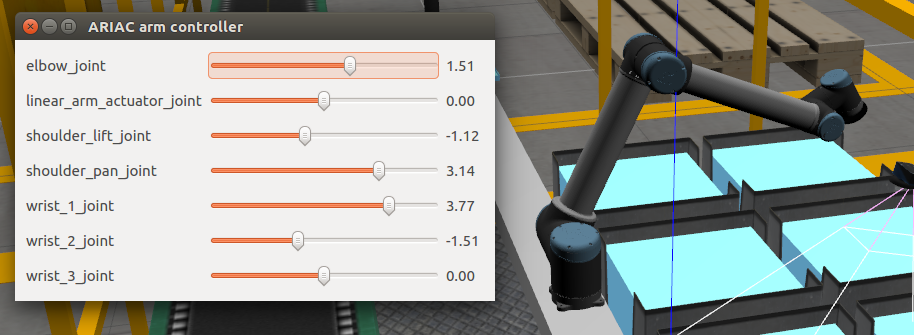
\includegraphics[width=0.7\textwidth]{mando.png}
	\caption{Interfaz gráfica del controlador del brazo.}
	\label{fig:mando}
\end{figure}

En lugar de utilizar la interfaz gráfica proporcionada por Qt para construir nuestra GUI la escribimos directamente en código utilizando las propiedades de auto-colocación de objetos. Qt nos permite insertar los elementos como si de una tabla se tratase y automáticamente los separa y les dá un espacio suficiente para mostrarse completos. También resulta más fácil programar después el comportamiento de la interfaz, ya que tenemos un mayor control sobre lo que creamos. 

A la hora de crear el controlador agrupando todos los elementos, podemos organizar el código en base a si es relativo a la interfaz o a ROS, por lo que lo dividimos en dos carpetas dentro de la carpetaa principal: \textit{gui} y \textit{ros\_manager}. Organizamos todo el código necesario en cinco ficheros:
\begin{itemize}
	\item \textit{main.py}: Este fichero es el encargado de lanzar los procesos relativos a la interfaz y a ROS. Es, por tanto, el ejecutable que invocamos para abrir el controlador. Se encuentra en la carpeta principal, y lanza los hilos de ejecución tanto de ROS como de la interfaz.
	
	\item \textit{gui.py}: En este fichero se encuentran definidos los elementos de la interfaz gráfica, así como el comportamiento de los mismos. Aquí creamos cada elemento, lo colocamos en la ventana, definimos los \textit{callbacks} de los deslizadores y capturamos el cierre de la ventana para realizar un cierre ordenado. Los \textit{callbacks} nos permiten capturar el movimiento de cada deslizador, actualizar la etiqueta correspondiente y enviar el nuevo valor al brazo. El cierre ordenado es necesario para poder cerrar el nodo de ROS y no dejar elementos corriendo en el sistema.
	
	\item \textit{threadGUI.py}: Este fichero crea un hilo de ejecución para los elementos de la interfaz gráfica. Dado que este elemento es común a todas las ventanas creadas con Qt, usamos el proporcionado en los tutoriales.
	
	\item \textit{ros.py}: En este fichero se encuentra el código relativo a ROS, el que gestiona el envío y recepción de mensajes. Aquí creamos el nodo, nos subscribimos al brazo, publicamos en él, gestionamos los cambios de posición de los deslizadores de la ventana y controlamos el cierre ordenado del nodo ROS.
	
	\item \textit{threadPublisher.py}: Este fichero crea un hilo de ejecución para los elementos de ROS. Dado que no es nuevo ni único para nuestro proyecto, reutilizamos uno de los usados en otros controladores de JdeRobot, simplemente cambiando el objeto de control del hilo.
	
\end{itemize}

En la Figura \ref{fig:mando} podemos ver la apariencia final del controlador del brazo.







sección moveit

















	
\begin{thebibliography}{99}
\bibitem{wikipedia} Página oficial de Wikipedia: \url{https://www.wikipedia.org/}
\bibitem{github} Página oficial de GitHub: \url{https://github.com/}
\bibitem{git} Página oficial de Git: \url{https://git-scm.com/}
\bibitem{blender} Página oficial de Blender: \url{https://www.blender.org/}
\bibitem{gazebo} Página oficial de Gazebo: \url{http://gazebosim.org/}
\bibitem{jderobot} Página oficial de JdeRobot: \url{http://jderobot.org/Main_Page}
\bibitem{ariac} Página oficial de ARIAC: \url{http://gazebosim.org/ariac}
\bibitem{ariacwiki} Página oficial de documentación de ARIAC: \url{https://bitbucket.org/osrf/ariac/wiki/Home}
\bibitem{ros} Página oficial de ROS: \url{http://www.ros.org/}
\bibitem{roswiki} Página oficial de documentación de ROS: \url{http://wiki.ros.org/}
\bibitem{moveit} Página oficial de MoveIt: \url{http://moveit.ros.org/}
\bibitem{rviz} Página oficial de rViz: \url{http://wiki.ros.org/rviz}
\bibitem{rqt} Página oficial de rqt: \url{http://wiki.ros.org/rqt}
\bibitem{texturescom} Página de texturas: \url{https://www.textures.com/}
\bibitem{qt} Página oficial de Qt: \url{https://www.qt.io/es/}
\end{thebibliography} 
	

\end{document}